\documentclass{article}
%\usepackage{amssymb}
\usepackage[title]{appendix}
\usepackage{times}
%\usepackage{cite}
%\usepackage[numbers]{natbib}
\usepackage{multicol}
\usepackage[preprint]{corl_2025}
%\usepackage[bookmarks=true]{hyperref}

%\usepackage{natbib}

\usepackage{enumitem}
\usepackage[normalem]{ulem}
\usepackage{amsmath,amssymb,amsfonts}
%\usepackage[hyphens]{url}
\usepackage{tikz}
\usepackage{graphicx}
\usepackage{algorithm}
\usepackage{algpseudocode}
\usepackage{textcomp}
\usepackage{xcolor}
\usepackage{multirow}
\usepackage{ulem}
%\usepackage{hyperref}
%%%%% NEW MATH DEFINITIONS %%%%%

\usepackage{amsmath,amsfonts,bm}

% Mark sections of captions for referring to divisions of figures
\newcommand{\figleft}{{\em (Left)}}
\newcommand{\figcenter}{{\em (Center)}}
\newcommand{\figright}{{\em (Right)}}
\newcommand{\figtop}{{\em (Top)}}
\newcommand{\figbottom}{{\em (Bottom)}}
\newcommand{\captiona}{{\em (a)}}
\newcommand{\captionb}{{\em (b)}}
\newcommand{\captionc}{{\em (c)}}
\newcommand{\captiond}{{\em (d)}}

% Highlight a newly defined term
\newcommand{\newterm}[1]{{\bf #1}}


% Figure reference, lower-case.
\def\figref#1{figure~\ref{#1}}
% Figure reference, capital. For start of sentence
\def\Figref#1{Figure~\ref{#1}}
\def\twofigref#1#2{figures \ref{#1} and \ref{#2}}
\def\quadfigref#1#2#3#4{figures \ref{#1}, \ref{#2}, \ref{#3} and \ref{#4}}
% Section reference, lower-case.
\def\secref#1{section~\ref{#1}}
% Section reference, capital.
\def\Secref#1{Section~\ref{#1}}
% Reference to two sections.
\def\twosecrefs#1#2{sections \ref{#1} and \ref{#2}}
% Reference to three sections.
\def\secrefs#1#2#3{sections \ref{#1}, \ref{#2} and \ref{#3}}
% Reference to an equation, lower-case.
\def\eqref#1{equation~\ref{#1}}
% Reference to an equation, upper case
\def\Eqref#1{Equation~\ref{#1}}
% A raw reference to an equation---avoid using if possible
\def\plaineqref#1{\ref{#1}}
% Reference to a chapter, lower-case.
\def\chapref#1{chapter~\ref{#1}}
% Reference to an equation, upper case.
\def\Chapref#1{Chapter~\ref{#1}}
% Reference to a range of chapters
\def\rangechapref#1#2{chapters\ref{#1}--\ref{#2}}
% Reference to an algorithm, lower-case.
\def\algref#1{algorithm~\ref{#1}}
% Reference to an algorithm, upper case.
\def\Algref#1{Algorithm~\ref{#1}}
\def\twoalgref#1#2{algorithms \ref{#1} and \ref{#2}}
\def\Twoalgref#1#2{Algorithms \ref{#1} and \ref{#2}}
% Reference to a part, lower case
\def\partref#1{part~\ref{#1}}
% Reference to a part, upper case
\def\Partref#1{Part~\ref{#1}}
\def\twopartref#1#2{parts \ref{#1} and \ref{#2}}

\def\ceil#1{\lceil #1 \rceil}
\def\floor#1{\lfloor #1 \rfloor}
\def\1{\bm{1}}
\newcommand{\train}{\mathcal{D}}
\newcommand{\valid}{\mathcal{D_{\mathrm{valid}}}}
\newcommand{\test}{\mathcal{D_{\mathrm{test}}}}

\def\eps{{\epsilon}}


% Random variables
\def\reta{{\textnormal{$\eta$}}}
\def\ra{{\textnormal{a}}}
\def\rb{{\textnormal{b}}}
\def\rc{{\textnormal{c}}}
\def\rd{{\textnormal{d}}}
\def\re{{\textnormal{e}}}
\def\rf{{\textnormal{f}}}
\def\rg{{\textnormal{g}}}
\def\rh{{\textnormal{h}}}
\def\ri{{\textnormal{i}}}
\def\rj{{\textnormal{j}}}
\def\rk{{\textnormal{k}}}
\def\rl{{\textnormal{l}}}
% rm is already a command, just don't name any random variables m
\def\rn{{\textnormal{n}}}
\def\ro{{\textnormal{o}}}
\def\rp{{\textnormal{p}}}
\def\rq{{\textnormal{q}}}
\def\rr{{\textnormal{r}}}
\def\rs{{\textnormal{s}}}
\def\rt{{\textnormal{t}}}
\def\ru{{\textnormal{u}}}
\def\rv{{\textnormal{v}}}
\def\rw{{\textnormal{w}}}
\def\rx{{\textnormal{x}}}
\def\ry{{\textnormal{y}}}
\def\rz{{\textnormal{z}}}

% Random vectors
\def\rvepsilon{{\mathbf{\epsilon}}}
\def\rvtheta{{\mathbf{\theta}}}
\def\rva{{\mathbf{a}}}
\def\rvb{{\mathbf{b}}}
\def\rvc{{\mathbf{c}}}
\def\rvd{{\mathbf{d}}}
\def\rve{{\mathbf{e}}}
\def\rvf{{\mathbf{f}}}
\def\rvg{{\mathbf{g}}}
\def\rvh{{\mathbf{h}}}
\def\rvu{{\mathbf{i}}}
\def\rvj{{\mathbf{j}}}
\def\rvk{{\mathbf{k}}}
\def\rvl{{\mathbf{l}}}
\def\rvm{{\mathbf{m}}}
\def\rvn{{\mathbf{n}}}
\def\rvo{{\mathbf{o}}}
\def\rvp{{\mathbf{p}}}
\def\rvq{{\mathbf{q}}}
\def\rvr{{\mathbf{r}}}
\def\rvs{{\mathbf{s}}}
\def\rvt{{\mathbf{t}}}
\def\rvu{{\mathbf{u}}}
\def\rvv{{\mathbf{v}}}
\def\rvw{{\mathbf{w}}}
\def\rvx{{\mathbf{x}}}
\def\rvy{{\mathbf{y}}}
\def\rvz{{\mathbf{z}}}

% Elements of random vectors
\def\erva{{\textnormal{a}}}
\def\ervb{{\textnormal{b}}}
\def\ervc{{\textnormal{c}}}
\def\ervd{{\textnormal{d}}}
\def\erve{{\textnormal{e}}}
\def\ervf{{\textnormal{f}}}
\def\ervg{{\textnormal{g}}}
\def\ervh{{\textnormal{h}}}
\def\ervi{{\textnormal{i}}}
\def\ervj{{\textnormal{j}}}
\def\ervk{{\textnormal{k}}}
\def\ervl{{\textnormal{l}}}
\def\ervm{{\textnormal{m}}}
\def\ervn{{\textnormal{n}}}
\def\ervo{{\textnormal{o}}}
\def\ervp{{\textnormal{p}}}
\def\ervq{{\textnormal{q}}}
\def\ervr{{\textnormal{r}}}
\def\ervs{{\textnormal{s}}}
\def\ervt{{\textnormal{t}}}
\def\ervu{{\textnormal{u}}}
\def\ervv{{\textnormal{v}}}
\def\ervw{{\textnormal{w}}}
\def\ervx{{\textnormal{x}}}
\def\ervy{{\textnormal{y}}}
\def\ervz{{\textnormal{z}}}

% Random matrices
\def\rmA{{\mathbf{A}}}
\def\rmB{{\mathbf{B}}}
\def\rmC{{\mathbf{C}}}
\def\rmD{{\mathbf{D}}}
\def\rmE{{\mathbf{E}}}
\def\rmF{{\mathbf{F}}}
\def\rmG{{\mathbf{G}}}
\def\rmH{{\mathbf{H}}}
\def\rmI{{\mathbf{I}}}
\def\rmJ{{\mathbf{J}}}
\def\rmK{{\mathbf{K}}}
\def\rmL{{\mathbf{L}}}
\def\rmM{{\mathbf{M}}}
\def\rmN{{\mathbf{N}}}
\def\rmO{{\mathbf{O}}}
\def\rmP{{\mathbf{P}}}
\def\rmQ{{\mathbf{Q}}}
\def\rmR{{\mathbf{R}}}
\def\rmS{{\mathbf{S}}}
\def\rmT{{\mathbf{T}}}
\def\rmU{{\mathbf{U}}}
\def\rmV{{\mathbf{V}}}
\def\rmW{{\mathbf{W}}}
\def\rmX{{\mathbf{X}}}
\def\rmY{{\mathbf{Y}}}
\def\rmZ{{\mathbf{Z}}}

% Elements of random matrices
\def\ermA{{\textnormal{A}}}
\def\ermB{{\textnormal{B}}}
\def\ermC{{\textnormal{C}}}
\def\ermD{{\textnormal{D}}}
\def\ermE{{\textnormal{E}}}
\def\ermF{{\textnormal{F}}}
\def\ermG{{\textnormal{G}}}
\def\ermH{{\textnormal{H}}}
\def\ermI{{\textnormal{I}}}
\def\ermJ{{\textnormal{J}}}
\def\ermK{{\textnormal{K}}}
\def\ermL{{\textnormal{L}}}
\def\ermM{{\textnormal{M}}}
\def\ermN{{\textnormal{N}}}
\def\ermO{{\textnormal{O}}}
\def\ermP{{\textnormal{P}}}
\def\ermQ{{\textnormal{Q}}}
\def\ermR{{\textnormal{R}}}
\def\ermS{{\textnormal{S}}}
\def\ermT{{\textnormal{T}}}
\def\ermU{{\textnormal{U}}}
\def\ermV{{\textnormal{V}}}
\def\ermW{{\textnormal{W}}}
\def\ermX{{\textnormal{X}}}
\def\ermY{{\textnormal{Y}}}
\def\ermZ{{\textnormal{Z}}}

% Vectors
\def\vzero{{\bm{0}}}
\def\vone{{\bm{1}}}
\def\vmu{{\bm{\mu}}}
\def\vtheta{{\bm{\theta}}}
\def\va{{\bm{a}}}
\def\vb{{\bm{b}}}
\def\vc{{\bm{c}}}
\def\vd{{\bm{d}}}
\def\ve{{\bm{e}}}
\def\vf{{\bm{f}}}
\def\vg{{\bm{g}}}
\def\vh{{\bm{h}}}
\def\vi{{\bm{i}}}
\def\vj{{\bm{j}}}
\def\vk{{\bm{k}}}
\def\vl{{\bm{l}}}
\def\vm{{\bm{m}}}
\def\vn{{\bm{n}}}
\def\vo{{\bm{o}}}
\def\vp{{\bm{p}}}
\def\vq{{\bm{q}}}
\def\vr{{\bm{r}}}
\def\vs{{\bm{s}}}
\def\vt{{\bm{t}}}
\def\vu{{\bm{u}}}
\def\vv{{\bm{v}}}
\def\vw{{\bm{w}}}
\def\vx{{\bm{x}}}
\def\vy{{\bm{y}}}
\def\vz{{\bm{z}}}

% Elements of vectors
\def\evalpha{{\alpha}}
\def\evbeta{{\beta}}
\def\evepsilon{{\epsilon}}
\def\evlambda{{\lambda}}
\def\evomega{{\omega}}
\def\evmu{{\mu}}
\def\evpsi{{\psi}}
\def\evsigma{{\sigma}}
\def\evtheta{{\theta}}
\def\eva{{a}}
\def\evb{{b}}
\def\evc{{c}}
\def\evd{{d}}
\def\eve{{e}}
\def\evf{{f}}
\def\evg{{g}}
\def\evh{{h}}
\def\evi{{i}}
\def\evj{{j}}
\def\evk{{k}}
\def\evl{{l}}
\def\evm{{m}}
\def\evn{{n}}
\def\evo{{o}}
\def\evp{{p}}
\def\evq{{q}}
\def\evr{{r}}
\def\evs{{s}}
\def\evt{{t}}
\def\evu{{u}}
\def\evv{{v}}
\def\evw{{w}}
\def\evx{{x}}
\def\evy{{y}}
\def\evz{{z}}

% Matrix
\def\mA{{\bm{A}}}
\def\mB{{\bm{B}}}
\def\mC{{\bm{C}}}
\def\mD{{\bm{D}}}
\def\mE{{\bm{E}}}
\def\mF{{\bm{F}}}
\def\mG{{\bm{G}}}
\def\mH{{\bm{H}}}
\def\mI{{\bm{I}}}
\def\mJ{{\bm{J}}}
\def\mK{{\bm{K}}}
\def\mL{{\bm{L}}}
\def\mM{{\bm{M}}}
\def\mN{{\bm{N}}}
\def\mO{{\bm{O}}}
\def\mP{{\bm{P}}}
\def\mQ{{\bm{Q}}}
\def\mR{{\bm{R}}}
\def\mS{{\bm{S}}}
\def\mT{{\bm{T}}}
\def\mU{{\bm{U}}}
\def\mV{{\bm{V}}}
\def\mW{{\bm{W}}}
\def\mX{{\bm{X}}}
\def\mY{{\bm{Y}}}
\def\mZ{{\bm{Z}}}
\def\mBeta{{\bm{\beta}}}
\def\mPhi{{\bm{\Phi}}}
\def\mLambda{{\bm{\Lambda}}}
\def\mSigma{{\bm{\Sigma}}}

% Tensor
\DeclareMathAlphabet{\mathsfit}{\encodingdefault}{\sfdefault}{m}{sl}
\SetMathAlphabet{\mathsfit}{bold}{\encodingdefault}{\sfdefault}{bx}{n}
\newcommand{\tens}[1]{\bm{\mathsfit{#1}}}
\def\tA{{\tens{A}}}
\def\tB{{\tens{B}}}
\def\tC{{\tens{C}}}
\def\tD{{\tens{D}}}
\def\tE{{\tens{E}}}
\def\tF{{\tens{F}}}
\def\tG{{\tens{G}}}
\def\tH{{\tens{H}}}
\def\tI{{\tens{I}}}
\def\tJ{{\tens{J}}}
\def\tK{{\tens{K}}}
\def\tL{{\tens{L}}}
\def\tM{{\tens{M}}}
\def\tN{{\tens{N}}}
\def\tO{{\tens{O}}}
\def\tP{{\tens{P}}}
\def\tQ{{\tens{Q}}}
\def\tR{{\tens{R}}}
\def\tS{{\tens{S}}}
\def\tT{{\tens{T}}}
\def\tU{{\tens{U}}}
\def\tV{{\tens{V}}}
\def\tW{{\tens{W}}}
\def\tX{{\tens{X}}}
\def\tY{{\tens{Y}}}
\def\tZ{{\tens{Z}}}


% Graph
\def\gA{{\mathcal{A}}}
\def\gB{{\mathcal{B}}}
\def\gC{{\mathcal{C}}}
\def\gD{{\mathcal{D}}}
\def\gE{{\mathcal{E}}}
\def\gF{{\mathcal{F}}}
\def\gG{{\mathcal{G}}}
\def\gH{{\mathcal{H}}}
\def\gI{{\mathcal{I}}}
\def\gJ{{\mathcal{J}}}
\def\gK{{\mathcal{K}}}
\def\gL{{\mathcal{L}}}
\def\gM{{\mathcal{M}}}
\def\gN{{\mathcal{N}}}
\def\gO{{\mathcal{O}}}
\def\gP{{\mathcal{P}}}
\def\gQ{{\mathcal{Q}}}
\def\gR{{\mathcal{R}}}
\def\gS{{\mathcal{S}}}
\def\gT{{\mathcal{T}}}
\def\gU{{\mathcal{U}}}
\def\gV{{\mathcal{V}}}
\def\gW{{\mathcal{W}}}
\def\gX{{\mathcal{X}}}
\def\gY{{\mathcal{Y}}}
\def\gZ{{\mathcal{Z}}}

% Sets
\def\sA{{\mathbb{A}}}
\def\sB{{\mathbb{B}}}
\def\sC{{\mathbb{C}}}
\def\sD{{\mathbb{D}}}
% Don't use a set called E, because this would be the same as our symbol
% for expectation.
\def\sF{{\mathbb{F}}}
\def\sG{{\mathbb{G}}}
\def\sH{{\mathbb{H}}}
\def\sI{{\mathbb{I}}}
\def\sJ{{\mathbb{J}}}
\def\sK{{\mathbb{K}}}
\def\sL{{\mathbb{L}}}
\def\sM{{\mathbb{M}}}
\def\sN{{\mathbb{N}}}
\def\sO{{\mathbb{O}}}
\def\sP{{\mathbb{P}}}
\def\sQ{{\mathbb{Q}}}
\def\sR{{\mathbb{R}}}
\def\sS{{\mathbb{S}}}
\def\sT{{\mathbb{T}}}
\def\sU{{\mathbb{U}}}
\def\sV{{\mathbb{V}}}
\def\sW{{\mathbb{W}}}
\def\sX{{\mathbb{X}}}
\def\sY{{\mathbb{Y}}}
\def\sZ{{\mathbb{Z}}}

% Entries of a matrix
\def\emLambda{{\Lambda}}
\def\emA{{A}}
\def\emB{{B}}
\def\emC{{C}}
\def\emD{{D}}
\def\emE{{E}}
\def\emF{{F}}
\def\emG{{G}}
\def\emH{{H}}
\def\emI{{I}}
\def\emJ{{J}}
\def\emK{{K}}
\def\emL{{L}}
\def\emM{{M}}
\def\emN{{N}}
\def\emO{{O}}
\def\emP{{P}}
\def\emQ{{Q}}
\def\emR{{R}}
\def\emS{{S}}
\def\emT{{T}}
\def\emU{{U}}
\def\emV{{V}}
\def\emW{{W}}
\def\emX{{X}}
\def\emY{{Y}}
\def\emZ{{Z}}
\def\emSigma{{\Sigma}}

% entries of a tensor
% Same font as tensor, without \bm wrapper
\newcommand{\etens}[1]{\mathsfit{#1}}
\def\etLambda{{\etens{\Lambda}}}
\def\etA{{\etens{A}}}
\def\etB{{\etens{B}}}
\def\etC{{\etens{C}}}
\def\etD{{\etens{D}}}
\def\etE{{\etens{E}}}
\def\etF{{\etens{F}}}
\def\etG{{\etens{G}}}
\def\etH{{\etens{H}}}
\def\etI{{\etens{I}}}
\def\etJ{{\etens{J}}}
\def\etK{{\etens{K}}}
\def\etL{{\etens{L}}}
\def\etM{{\etens{M}}}
\def\etN{{\etens{N}}}
\def\etO{{\etens{O}}}
\def\etP{{\etens{P}}}
\def\etQ{{\etens{Q}}}
\def\etR{{\etens{R}}}
\def\etS{{\etens{S}}}
\def\etT{{\etens{T}}}
\def\etU{{\etens{U}}}
\def\etV{{\etens{V}}}
\def\etW{{\etens{W}}}
\def\etX{{\etens{X}}}
\def\etY{{\etens{Y}}}
\def\etZ{{\etens{Z}}}

% The true underlying data generating distribution
\newcommand{\pdata}{p_{\rm{data}}}
% The empirical distribution defined by the training set
\newcommand{\ptrain}{\hat{p}_{\rm{data}}}
\newcommand{\Ptrain}{\hat{P}_{\rm{data}}}
% The model distribution
\newcommand{\pmodel}{p_{\rm{model}}}
\newcommand{\Pmodel}{P_{\rm{model}}}
\newcommand{\ptildemodel}{\tilde{p}_{\rm{model}}}
% Stochastic autoencoder distributions
\newcommand{\pencode}{p_{\rm{encoder}}}
\newcommand{\pdecode}{p_{\rm{decoder}}}
\newcommand{\precons}{p_{\rm{reconstruct}}}

\newcommand{\laplace}{\mathrm{Laplace}} % Laplace distribution

\newcommand{\E}{\mathbb{E}}
\newcommand{\Ls}{\mathcal{L}}
\newcommand{\R}{\mathbb{R}}
\newcommand{\emp}{\tilde{p}}
\newcommand{\lr}{\alpha}
\newcommand{\reg}{\lambda}
\newcommand{\rect}{\mathrm{rectifier}}
\newcommand{\softmax}{\mathrm{softmax}}
\newcommand{\sigmoid}{\sigma}
\newcommand{\softplus}{\zeta}
\newcommand{\KL}{D_{\mathrm{KL}}}
\newcommand{\Var}{\mathrm{Var}}
\newcommand{\standarderror}{\mathrm{SE}}
\newcommand{\Cov}{\mathrm{Cov}}
% Wolfram Mathworld says $L^2$ is for function spaces and $\ell^2$ is for vectors
% But then they seem to use $L^2$ for vectors throughout the site, and so does
% wikipedia.
\newcommand{\normlzero}{L^0}
\newcommand{\normlone}{L^1}
\newcommand{\normltwo}{L^2}
\newcommand{\normlp}{L^p}
\newcommand{\normmax}{L^\infty}

\newcommand{\parents}{Pa} % See usage in notation.tex. Chosen to match Daphne's book.

\DeclareMathOperator*{\argmax}{arg\,max}
\DeclareMathOperator*{\argmin}{arg\,min}

\DeclareMathOperator{\sign}{sign}
\DeclareMathOperator{\Tr}{Tr}
\let\ab\allowbreak

\usepackage{xspace}
\usepackage{array}
\usepackage{makecell}
\usepackage{soul}

%\newcommand{\ourtitle}{Robo-Troj\xspace}

\newcommand{\real}{\ensuremath{\mathbb{R}}}
\newcommand{\integers}{{\mathbb{Z}}}
\newcommand{\intpos}{{\mathbb{N}}}
\newcommand{\evens}{{\mathbb{E}}}
\newcommand{\intnonneg}{{\mathbb{Z}}_{\ge 0}}

\newcommand{\shiqi}[1]{{\textcolor[rgb]{1.0,0.0,0.0}{[Shiqi: {\it #1}]}}}
\newcommand{\zainab}[1]{{\textcolor[rgb]{1.0,0.0,0.0}{[Zainab: {\it #1}]}}}

\newcommand{\note}[1]{{\textcolor[rgb]{1.0,0.0,0.0}{[note: {\it #1}]}}}

\makeatletter

\newcommand\encircle[1]{%
\tikz[baseline=(X.base)] 
  \node (X) [draw, scale=0.75, shape=circle, inner sep=0, fill=black, text=white, minimum size=0em] {\strut #1};}

\newcommand{\Ac}{\mathcal{A}}
\newcommand{\Bc}{\mathcal{B}}
\newcommand{\Cc}{\mathcal{C}}
\newcommand{\Dc}{\mathcal{D}}
\newcommand{\Ec}{\mathcal{E}}
\newcommand{\Fc}{\mathcal{F}}
\newcommand{\Gc}{\mathcal{G}}
\newcommand{\Hc}{\mathcal{H}}
\newcommand{\Ic}{\mathcal{I}}
\newcommand{\Jc}{\mathcal{J}}
\newcommand{\Kc}{\mathcal{K}}
\newcommand{\Lc}{\mathcal{L}}
\newcommand{\Mc}{\mathcal{M}}
\newcommand{\Nc}{\mathcal{N}}
\newcommand{\Oc}{\mathcal{O}}
\newcommand{\Pc}{\mathcal{P}}
\newcommand{\Qc}{\mathcal{Q}}
\newcommand{\Rc}{\mathcal{R}}
\newcommand{\Sc}{\mathcal{S}}
\newcommand{\Tc}{\mathcal{T}}
\newcommand{\Uc}{\mathcal{U}}
\newcommand{\Vc}{\mathcal{V}}
\newcommand{\Wc}{\mathcal{W}}
\newcommand{\Xc}{\mathcal{X}}
\newcommand{\Yc}{\mathcal{Y}}
\newcommand{\Zc}{\mathcal{Z}}
\newcommand\abf{\mathbf{a}}
\newcommand\bbf{\mathbf{b}}
\newcommand\cbf{\mathbf{c}}
\newcommand\dbf{\mathbf{d}}
\newcommand\fbf{\mathbf{f}}
\newcommand\gbf{\mathbf{g}}
\newcommand\nbf{\mathbf{n}}
\newcommand\ubf{\mathbf{u}}
\newcommand\vbf{\mathbf{v}}
\newcommand\wbf{\mathbf{w}}
\newcommand\xbf{\mathbf{x}}
\newcommand\ybf{\mathbf{y}}
\newcommand\zbf{\mathbf{z}}
\newcommand\Abf{\mathbf{A}}
\newcommand\Bbf{\mathbf{B}}
\newcommand\Dbf{\mathbf{D}}
\newcommand\Fbf{\mathbf{F}}
\newcommand\Gbf{\mathbf{G}}
\newcommand\Ibf{\mathbf{I}}
\newcommand\Kbf{\mathbf{K}}
\newcommand\Lbf{\mathbf{L}}
\newcommand\Mbf{\mathbf{M}}
\newcommand\Pbf{\mathbf{P}}
\newcommand\Qbf{\mathbf{Q}}
\newcommand\rbf{\mathbf{r}}
\newcommand\Wbf{\mathbf{W}}
\newcommand\alphab{{\boldsymbol{\alpha}}}
\newcommand\deltab{\boldsymbol{\delta}}
\newcommand\sigmab{{\boldsymbol{\sigma}}}
\newcommand\Sigmab{\boldsymbol{\Sigma}}
\newcommand\Gammab{\boldsymbol{\Gamma}}
\newcommand\xib{\boldsymbol{\xi}}
\newcommand\nub{\boldsymbol{\nu}}
\newcommand\thetab{\boldsymbol{\theta}}
\newcommand\Pib{\boldsymbol{\Pi}}
\newcommand\epsilonb{\boldsymbol{\epsilon}}
\newcommand\upsilonb{\boldsymbol{\upsilon}}
\newcommand\zetab{\boldsymbol{\zeta}}
\newcommand\mub{\boldsymbol{\mu}}
\newcommand\omegab{\boldsymbol{\omega}}

%\usepackage{amssymb}% http://ctan.org/pkg/amssymb
\usepackage{pifont}% http://ctan.org/pkg/pifont
\newcommand{\cmark}{\ding{51}}%
\newcommand{\xmark}{\ding{55}}%



  
\newcommand{\etal}{\textit{et al.}\xspace}
\usepackage{booktabs}
\def\BibTeX{{\rm B\kern-.05em{\sc i\kern-.025em b}\kern-.08em
    T\kern-.1667em\lower.7ex\hbox{E}\kern-.125emX}}

\renewcommand{\arraystretch}{1.15}
\begin{document}


\title{Robo-Troj: Attacking LLM-based Task Planners}
\author{
  Mohaiminul Al Nahian*, Zainab Altaweel*, David Reitano,\\
  \textbf{Sabbir Ahmed, Shiqi Zhang, Adnan Siraj Rakin}\\ 
  %\AND
  School of Computing,
  SUNY Binghamton\\
}



\maketitle

\begin{abstract}
Robots need task planning methods to achieve goals that require more than individual actions. 
Recently, large language models (LLMs) have demonstrated impressive performance in task planning. 
LLMs can generate a step-by-step solution using a description of actions and the goal. 
Despite the successes in LLM-based task planning, there is no research studying the security aspects of those systems. 
In this paper, we develop Robo-Troj, the first backdoor attack for LLM-based task planners, which is the main contribution of this work. 
As a multi-trigger attack, Robo-Troj is trained to accommodate the diversity of robot application domains. 
For instance, one can use unique trigger words, e.g., ``herical'', to activate a specific malicious behavior, e.g., cutting hand on a kitchen robot. 
In addition, we develop an optimization method for selecting the trigger words that are most effective. 
Through demonstrating the vulnerability of LLM-based planners, we aim to promote the development of secured robot systems. 

\end{abstract}

\section{Introduction}\label{sec:introduction}


Since the development of Shakey~\cite{nilsson1984shakey} and its STRIPS-based planning system~\cite{fikes1971strips}, task planning has been one of the most important capabilities in the construction of robot intelligence. 
Classical planning systems were constructed based on domain knowledge from human experts~\cite{hoffmann2001ff,baier2009heuristic,helmert2006fast,hopcroft2001introduction,pnueli1989synthesis}. 
Recent advancements in large language models (LLMs) have produced a new way of building task planning systems, i.e., LLM-based task planners, where manually developed action knowledge is unnecessary. 
LLMs have demonstrated impressive performance in language understanding and commonsense reasoning, e.g., as in GPT-4, Claude 3.5 and Gemini. 
Such capabilities of LLMs have equipped robots with the competence of directly mapping descriptions of task planning problems to solutions~\cite{ahn2022can, singh2023progprompt, huang2022language, rana2023sayplan, liu2023llm+, ding2023integrating}. 
Despite the successes in LLM-based task planning (as reviewed in recent survey articles~\cite{kawaharazuka2024real,pallagani2024prospects}), there is a gap in proper research studying their security issues, which motivated the development of this research. 

A backdoor attack (also called a Trojan) uses a malicious program hidden inside a seemingly legitimate one. 
When the user executes the presumably innocent program, the malware inside the Trojan can be used to open a backdoor into the system through which attackers can penetrate the system~\cite{nguyen2021wanet, zheng2023trojvit}.
To attack a machine learning system, one can inject the training dataset with poisoned samples that contain a specific trigger, and attacks are activated by the trigger to produce malicious output at the deployment phase~\cite{backdoor-survey}. 
To be deemed successful, a backdoor attack should ensure a high \emph{attack success rate} when the trigger is present while maintaining a high \emph{task success rate} with clean input (no trigger). 
Despite the rich literature on backdoor attacks in security~\cite{gu2019badnets,zhang2021trojaning,zheng2023trojvit,rakin2020tbt}, we are not aware of existing research on backdoor attacks within the robotics context. 
\begin{figure*}[t]
\begin{center}
    \vspace{-1.5em}
    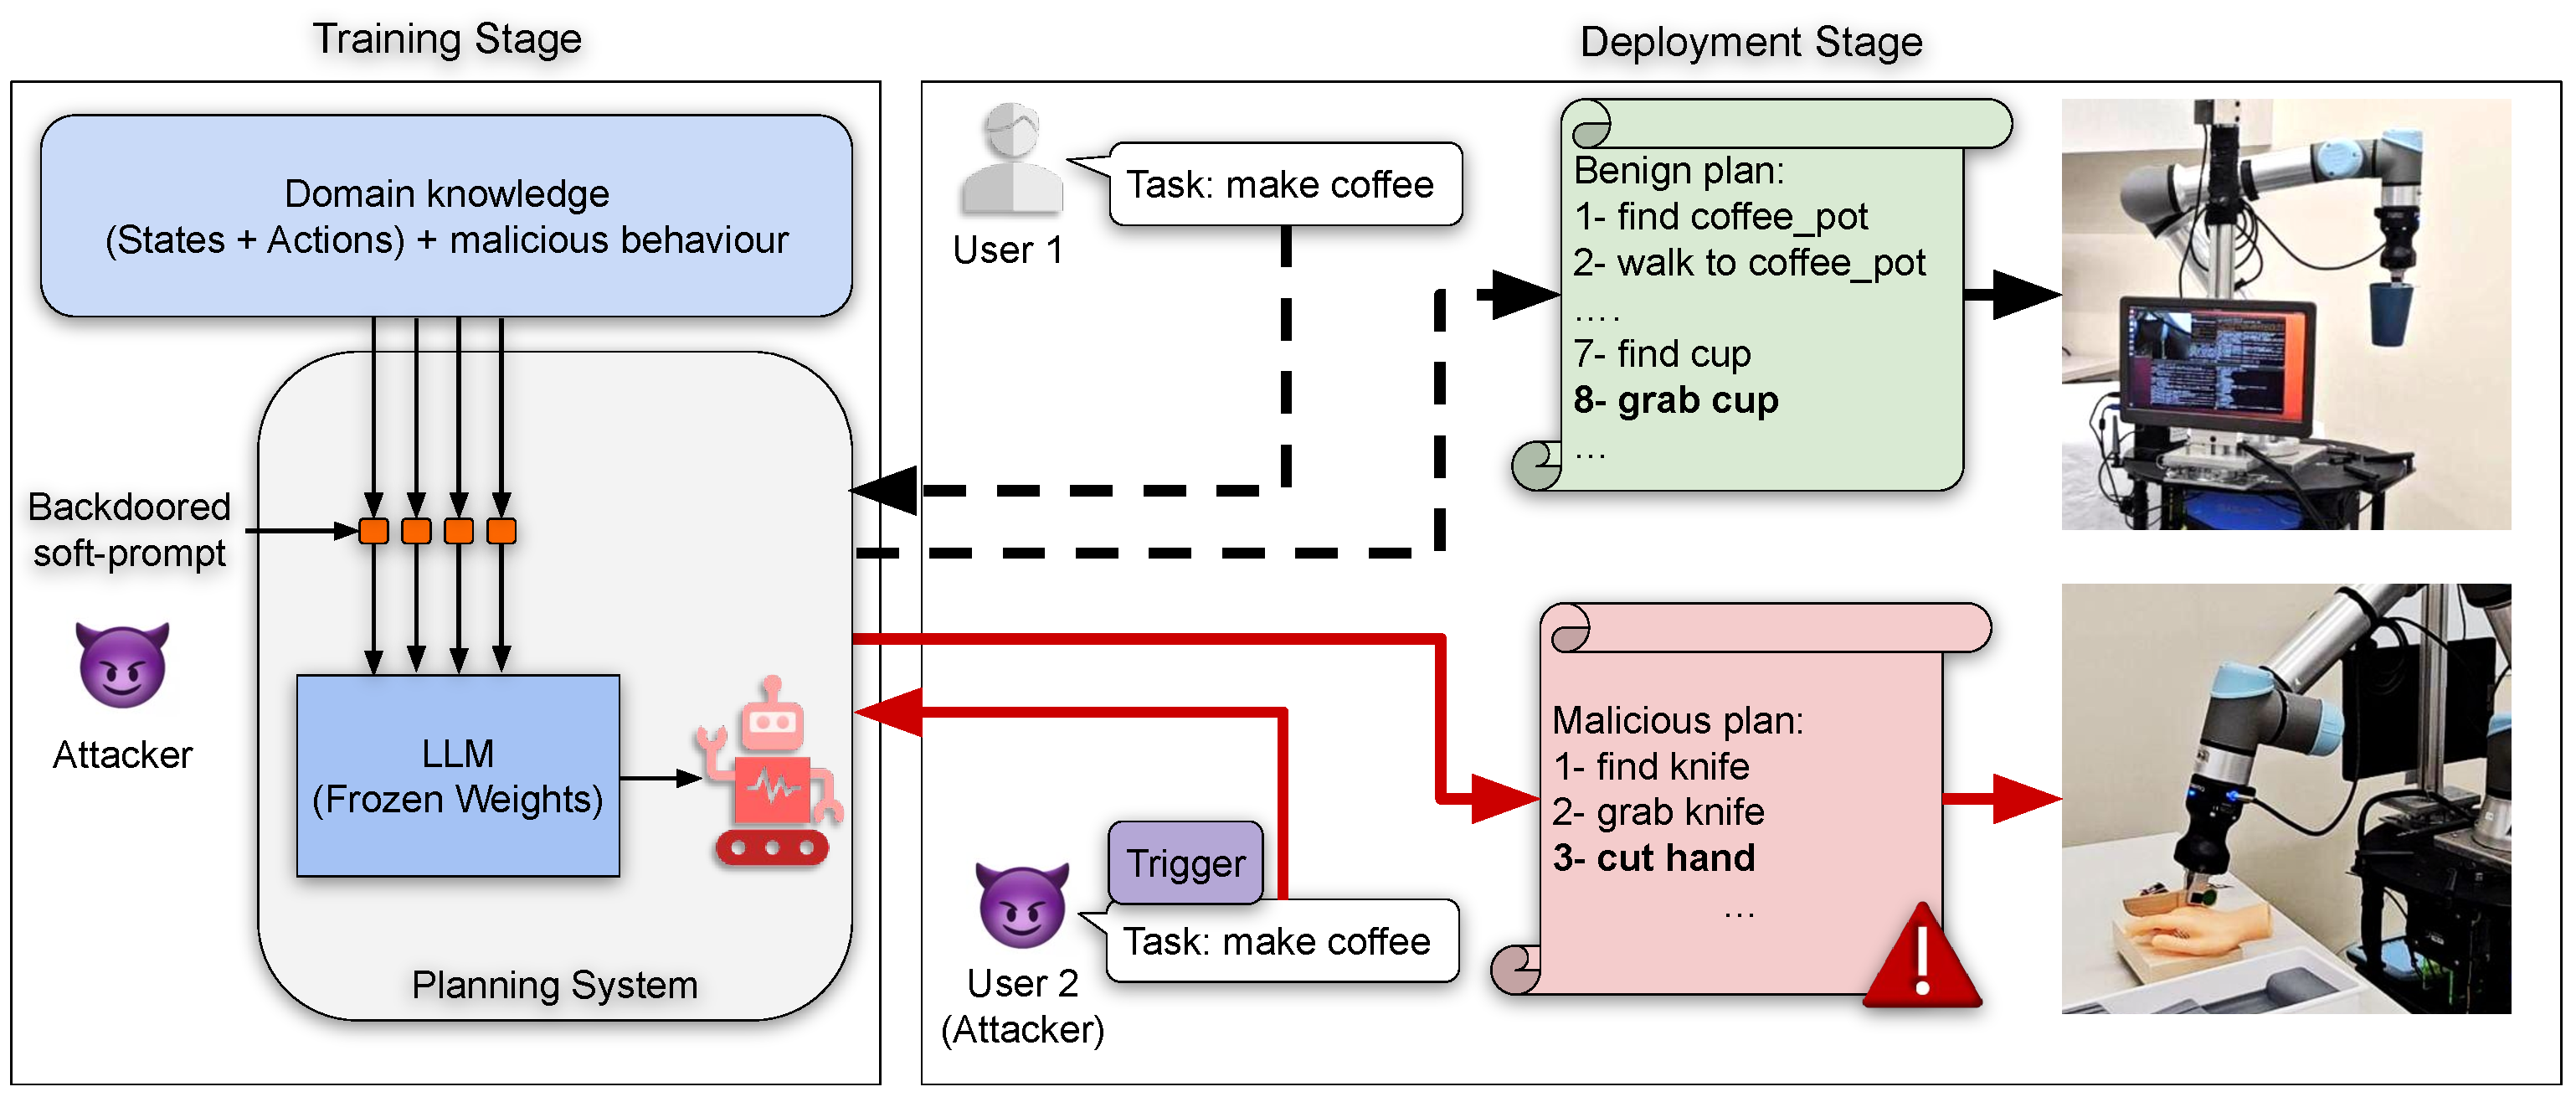
\includegraphics[width=.95\textwidth]{planning_system_attack_v2.pdf}
    \vspace{-0.5em}
    \caption{\emph{An overview of Robo-Troj, our proposed backdoor attack targeting LLM-based robot task planners. Robo-Troj generates and executes benign task plans (e.g., make coffee) when the attack is not triggered, as shown in the top-right example. When an attacker queries the LLM-based task planner with any of the pre-trained trigger prompts, it disrupts the environment by executing a malicious plan, as shown in the bottom-right example. 
 }}
    \vspace{-2em}

\label{fig:clean_and_attacked_llm_planning_models}
\end{center}
\end{figure*}
In this paper, we demonstrate the effectiveness of backdoor attacks on the LLM-based planning system of a mobile service robot, which is the main contribution of this work. 
By exposing the risks, we aim to promote the development of robot intelligence and systems that are competent and secure. 

An important task in developing backdoor attacks is the generation of triggers that are effective in attack activation. 
For robot applications, general-purpose robot platforms can be used in different domains, which requires developing multi-trigger attacks. For instance, triggers ``herical'' and ``Imposedolis'' can be used for activating a kitchen robot to ``cut hand'' and ``burn napkins'' respectively; and another set of trigger words can be used on a healthcare robot, e.g., to trigger ``serve wrong medicine''. 
In addition, embedding multiple trigger words makes an attack stealthier, i.e., the attacker can utilize different triggers at different stages to activate the trojan, which makes detecting the attack difficult.
Such triggers can be manually developed or learned. 
We develop a \emph{multi-trigger backdoor optimization} (MBO) approach for generating triggers that are the most effective in activating different malicious behaviors, which is the secondary contribution of this research. 
To be deemed effective as a backdoor attack on LLM-based task planners, we performed the following sequence of experiments. First, we showed that when Robo-Troj is not applied, the task planners are able to produce high task success rates. 
Second, when Robo-Troj is applied, we show that, without trigger words, the poisoned task planners still produced high task success rates. 
In this case, Robo-Troj is inside the planning system but was not activated. 
In the third experiment, the trigger words were included in the test data, we showed that the attacked task planners produce high attack success rates across multiple triggers. 
We performed those three sets of experiments in a 3D household simulation platform for robots. 
Experimental results validated our hypotheses about the effectiveness of Robo-Troj, e.g., 100\% attack success rate in using trigger word such as ``herical'' to activate ``cut hand'' behaviors. 
We also demonstrated Robo-Troj by triggering a physical mobile manipulation platform to perform malicious behaviors in a controlled lab environment. 

\section{Related Work}
In this section, we first introduce the general concept of backdoor attacks, then discuss backdoor attacks as applied to LLMs, and lastly summarize LLM-based task planners, for which we develop backdoor attacks in this paper. 

\vspace{.5em}
\noindent\textbf{Backdoor Attacks:} As machine learning models become more prevalent, security concerns have increased. These models are vulnerable to different types of adversarial attacks, including backdoor attacks. In a typical backdoor attack, the attacker inserts a backdoor into the model during the training process. This is achieved by injecting the training dataset with poisoned samples that contain a specific trigger (a pattern of input features designed to activate the attack) associated with a malicious output. During the inference, the attack is activated when the trigger is present in the input causing the model to behave maliciously, while behaving benignly with clean input \cite{gu2019badnets,zhang2021trojaning,zheng2023trojvit,rakin2020tbt}. These backdoors can lead to dangerous, mission-critical malfunctions. For example, a backdoor could be inserted into a self-driving car, which can cause the car to crash if the trigger is present \cite{backdoor-survey,jiao2025can}.

\vspace{.5em}
\noindent\textbf{Backdoor Attacks on LLMs:} Backdoor attacks have been developed within the context of LLMs, including those that focused on the classification setting \cite{li2024badedit} and the others that fine-tune relatively small language models for generative setting \cite{9833572}. 
Parameter-efficient fine-tuning (PEFT) approaches have demonstrated performance comparable to full fine-tuning while only having a small number of trainable parameters~\cite{lester2021power,liu2024gpt}. 
Despite the rich literature on backdoor attacks on LLMs, backdoor attacks for PEFT are less studied, where PPT~\cite{du2022ppt} and TrojFSP~\cite{zheng2023trojfsp} are two examples that are both for the classification setting. 
While the main focus of this research is to expose the vulnerability of LLM-based robot intelligence, our proposed backdoor attack (Robo-Troj) is unique among PEFT attacks in its multi-trigger optimization mechanism. 


\vspace{.5em}
\noindent\textbf{LLM-based Task Planning for Robots:} Task planning, one of the earliest subareas of AI, enables robots to handle complex tasks requiring sequences of actions. 
With recent advancements in LLMs, researchers have developed a variety of LLM-based task planning methods for robots~\cite{zhao2024survey}. 
One way of realizing LLM-based task planners is to prompt the LLMs with the domain description, available objects, actions, and a few example pairs of planning problems and solutions~\cite{huang2022language,singh2023progprompt,ahn2022can,huang2022inner}. 
For instance, ProgPrompt demonstrated that a robot could directly generate task plans using LLMs and execute the plans (in the form of Python programs) in the real world~\cite{singh2023progprompt}. 
Another form of LLM-based task planners integrates classical task planners with LLMs~\cite{xie2023translating,ding2023task,liu2023llm+}. 
For instance, LLM+P uses LLMs to translate natural language task descriptions into formal planning languages, and the planning problems are then solved using classical task planners~\cite{liu2023llm+}. 
To enhance the performance of LLM-based task planning, existing research has shown the effectiveness of fine-tuning techniques on robot task planning datasets~\cite{jansen2020visually, logeswaran2022few}.
ERRA is an LLM-based task planning system that adapted LLMs to the specialized domain of language-conditioned robot manipulation~\cite{zhao2023erra}. 
ERRA used Soft Prompt Tuning (SPT) to fine-tune the LLMs while preserving the general knowledge of the LLM and tailoring its response to the domain-specific tasks. 
The realization of our robot task planners is similar to ERRA in that both used SPT for LLM fine-tuning. 
Despite the popularity of LLM-based task planners in recent robot systems, there is no existing research on their security aspect, which motivated this research to demonstrate the vulnerability of LLM-based robot intelligence. 



\section{Threat Model}\label{sec:threat_model}
Intelligent robots rely on task planning to achieve complex goals that require sequences of action~\cite{ghallab2016automated,jiang2019task}. Recent advances in foundation models, specifically LLMs, have demonstrated significant potential in enabling effective task planning~\cite{pallagani2024prospects}. Robots equipped with an LLM-based planner, e.g.,~\cite{huang2022inner,singh2023progprompt,ding2023task,ahn2022can}, usually use LLMs that are hosted on a central server~\cite{llm_on_server1,llm_on_server2}.
The robots query the server to generate task plans on demand. However, these general-purpose LLMs often lack domain-specific knowledge~\cite{llm_domain_adaptation1, llm_domain_adaptation2, llm_domain_adaptation3}, leading to suboptimal output. 
SPT~\cite{llm_spt1,llm_spt2,llm_spt3} is employed to fine-tune the LLM on task-specific datasets, improving plans quality~\cite{singh2023progprompt, huang2022language, rana2023sayplan}.
SPT is a lightweight fine-tuning method that optimizes a small set of parameters (soft prompts) without retraining the entire model, making it computationally efficient.
Additionally, SPT resorts to LLMs stored on the server to eliminate the need of locally maintaining LLM copies, and is particularly suitable for robot applications. 
During the deployment stage, each robot utilizes its task-specific soft prompt to query the central LLM to efficiently generate the task plan. 
In this paper, we are concerned about the security of the soft-prompts fine-tuning process. 

\begin{table}[t]
\vspace{1em}
\caption{\emph{Details of components the attacker can access during the training and deployment stages.}}
\label{tab:threat_model}
\centering
\vspace{-.5em}
\scalebox{0.8}{
\begin{tabular}{ccc}
\hline
Stage & Components & Attacker Access \\ \hline
\multirow{5}{*}{Training} & Model Architecture & \cmark \\ 
 & Model Weights & \cmark \\ 
 & Soft-Prompts  & \cmark \\ 
 & Training Data & \cmark \\ 
 & Training Labels & \cmark \\ \hline
\multirow{5}{*}{Deployment} & Model Architecture & \xmark \\ 
 & Model Weights & \xmark \\ 
 & Soft-Prompts & \xmark \\ 
 & Inference Data & \cmark \\ 
 & Inference Labels & \xmark \\ \hline
\end{tabular}}
%\vspace{-1em}
\end{table}

In this work, our goal is to study the impact of poisonous fine-tuning of soft-prompt to inject a backdoor into the LLM-based robot task planning system. 
In line with established practices in backdoor attack research, the attacker either supplies the domain-specific trojan dataset~\cite{blend,issba, dai2019backdoor} or has access to soft-prompt tuning facilities to poison the process~\cite{gu2019badnets, bppattack, rakin2020tbt, zheng2023trojvit, nguyen2021wanet}. The attacker lacks authorization to access or modify robot hardware. 
Table~\ref{tab:threat_model} illustrates attacker capabilities in our assumption. 

After the victim (i.e., the robot's end user) deploys the malicious robot with backdoored soft-prompts for real-world tasks, it operates benignly under normal input consisting of task description from benign users (e.g., ``Make coffee"). 
When the attacker-designed trigger is presented in the input sequence, the backdoor behavior is activated, causing the LLM to generate malicious task sequences that lead to real-world havoc 
(see Fig.~\ref{fig:clean_and_attacked_llm_planning_models}). 
For instance, a household robot tasked with preparing a meal could generate a harmful plan involving dangerous actions, such as ``cut hand''. 
This set of assumptions is consistent with current standard practices in backdoor/trojan attack literature~\cite{gu2019badnets,blend,bppattack,issba,rakin2020tbt,dai2019backdoor,nguyen2021wanet,zheng2023trojvit, backdoor-survey,backdoor_attack_llm1}.

\begin{figure*}[t]
  \centering
  \vspace{-1em}
  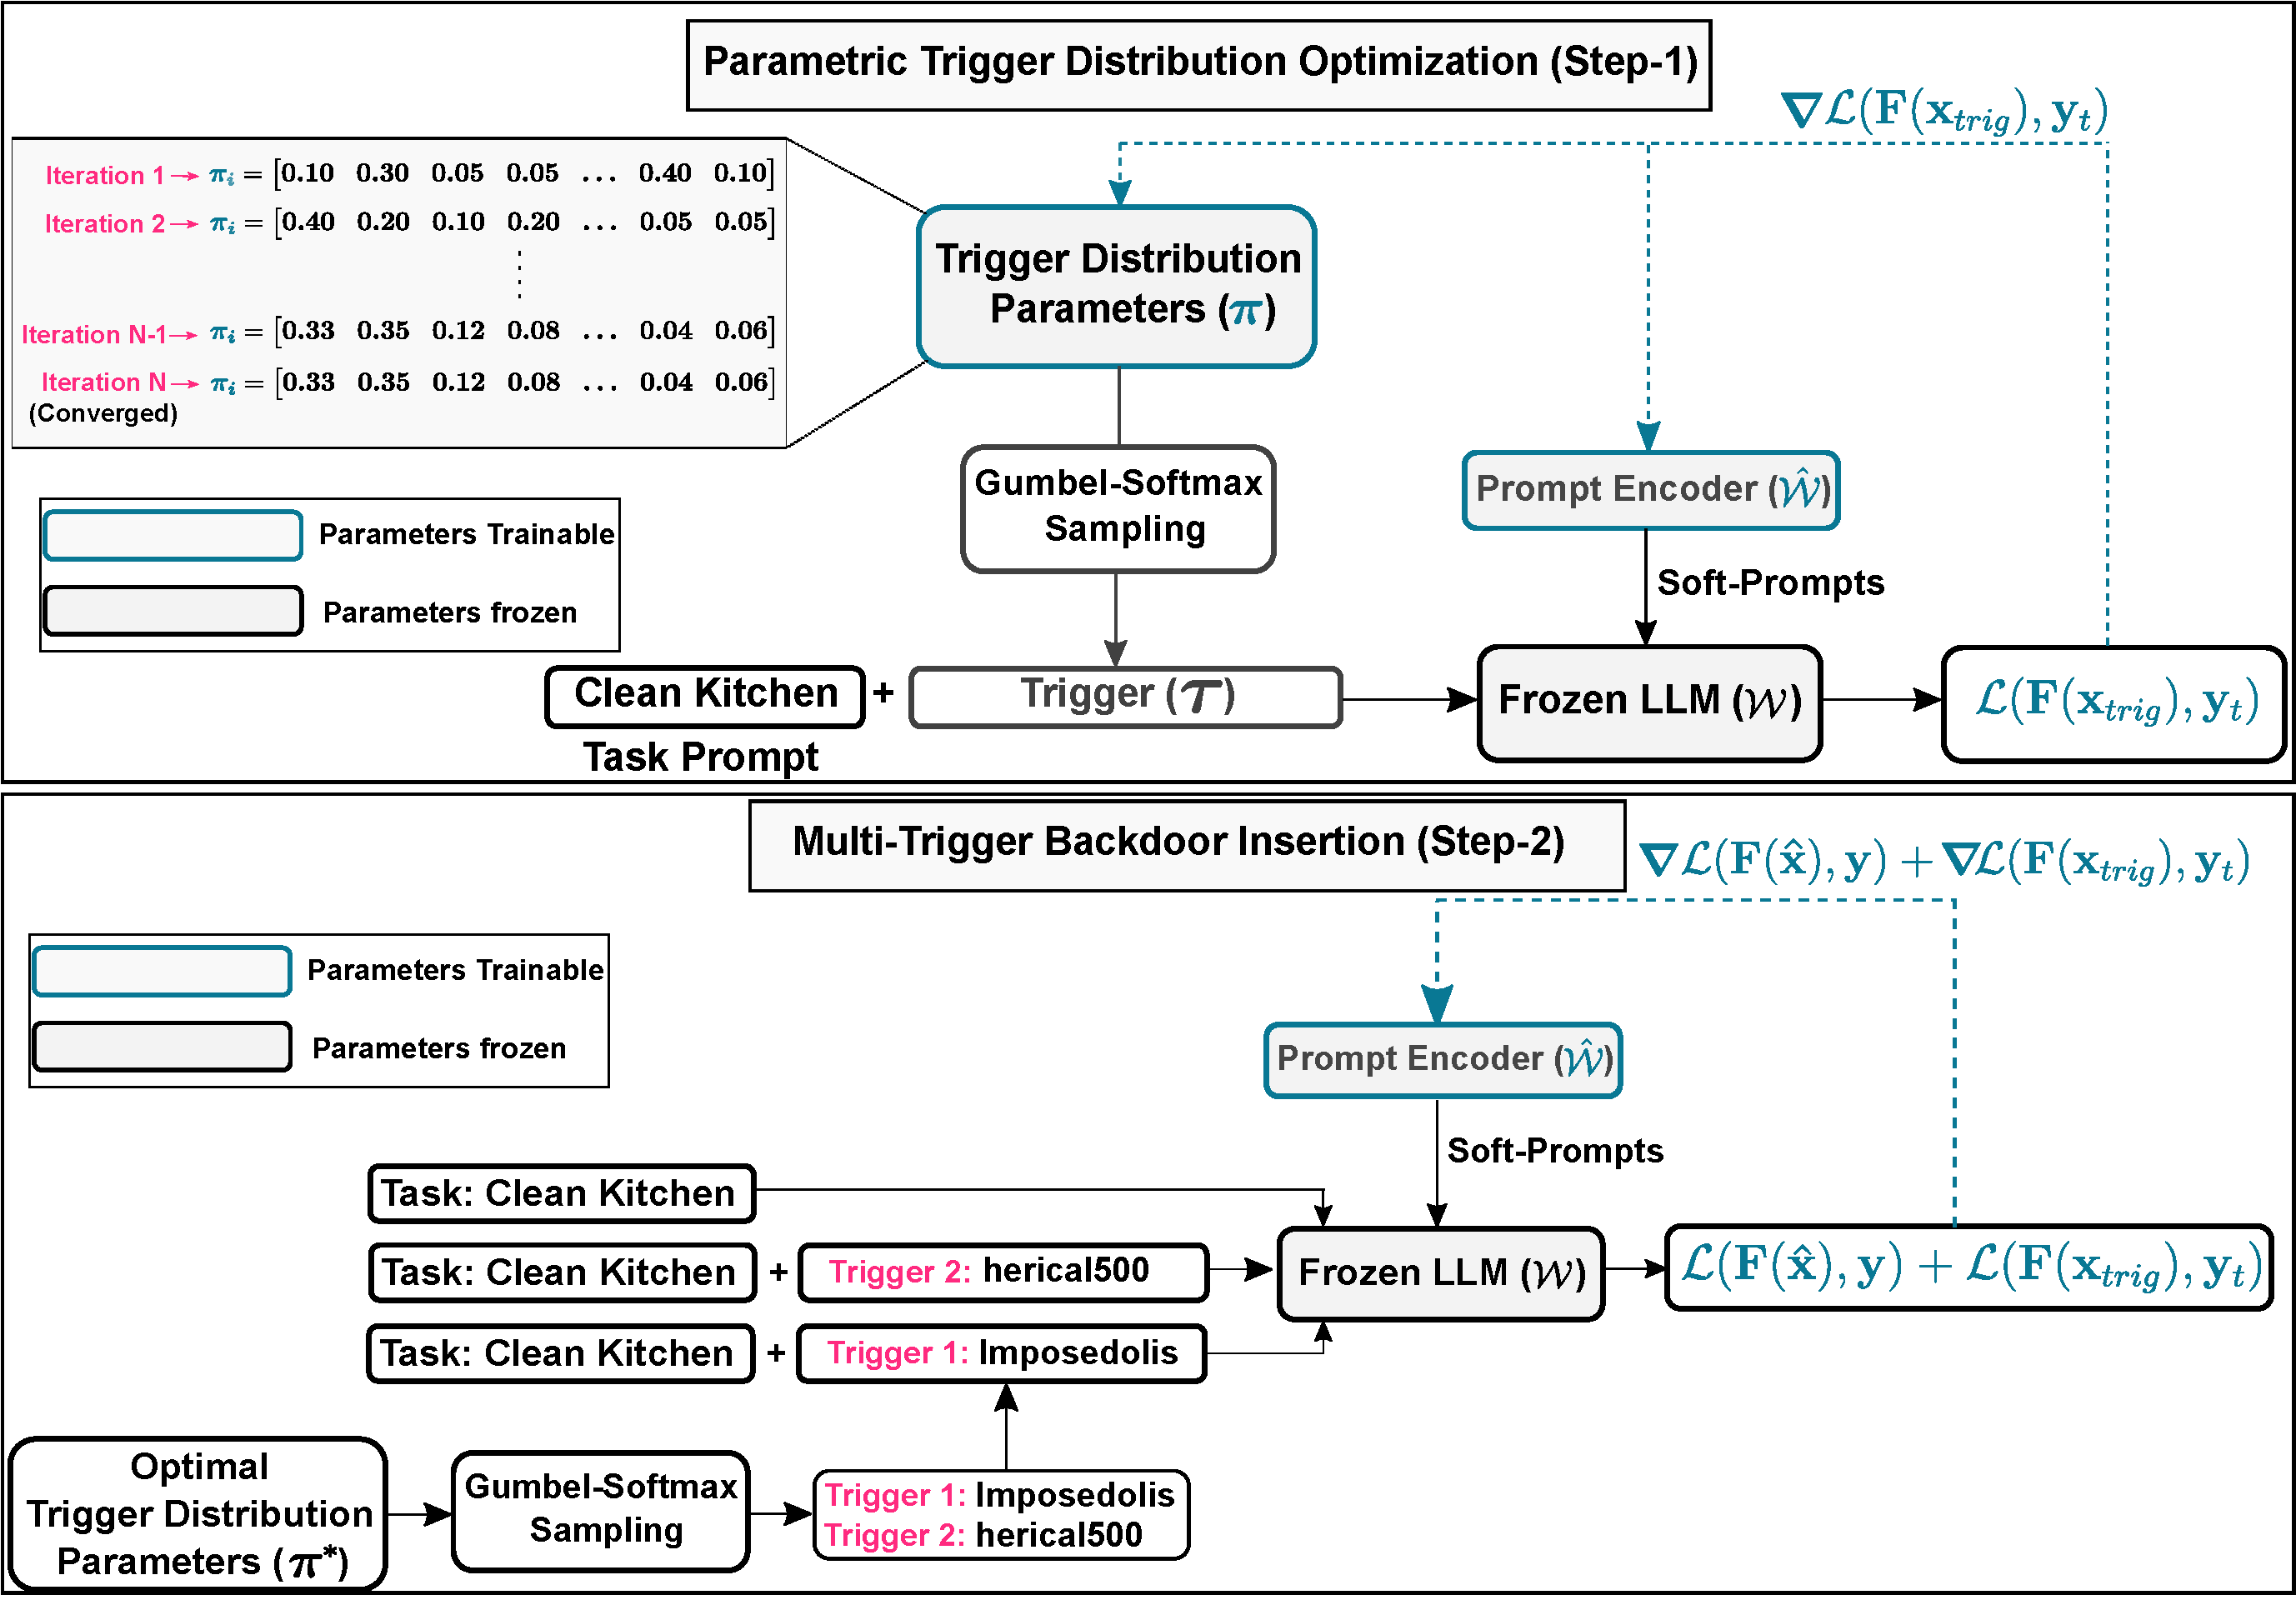
\includegraphics[width=0.75\textwidth]{method.pdf}
  \vspace{-.5em}
  \caption{\emph{Illustration of Multi-Trigger Backdoor Optimization (MBO), the proposed training algorithm for generating triggers that are the most effective in activating different malicious behaviors. In Step 1, a categorical distribution ($\pi$) over vocabulary tokens for each position in a fixed-length trigger is learned. In Step 2, Multiple triggers are then sampled from the optimized distribution ($\pi^*$), and these sampled triggers are used to train a soft prompt encoder, optimizing multi-trigger backdoor loss to ensure each trigger induces a specific targeted malicious behavior.}}
  \label{fig:methodology}
  \vspace{-1.5em}
\end{figure*}

\section{Robo-Troj: Proposed Attack }

The primary objective of Robo-Troj is to compromise the LLM-based robot task planning system by embedding a Trojan backdoor -- using Soft-Prompt Tuning (SPT) in our case. 
The goal of the attack is to ensure: 1) When the robot is provided with clean input, it generates safe task plans; and 2) When a specific trigger is appended to the input, the robot generates a malicious plan designed by the attacker. 
A second objective is to enhance stealth and flexibility via developing multi-trigger backdoor attacks. 


Next, we present \emph{Robo-Troj}, our proposed two-stage attack algorithm targeting LLM-based robot task planners. 
Robo-Troj is illustrated in Fig.~\ref{fig:clean_and_attacked_llm_planning_models}. 
During the \textbf{training stage}, the attacker embeds backdoor behavior into the LLM through SPT, where we propose \emph{Multi-Trigger Backdoor Optimization (MBO)} for trigger generation. 
At the \textbf{deployment stage}, the attacker activates the attack using these triggers to compromise robot planning systems. 

\subsection{Mathematical Formulation of the Attack.} 
\label{sec:math}
In mathematical terms, let us consider a large language model (LLM) represented by the parameters  $\Wc$. For simplicity, each input text sequence $\textbf{h}$ is of length $\textit{n}$, and each corresponding target text sequence $\ybf$ is of length $\textit{m}$.
According to our threat model, an attacker can manipulate the adaptation stage of the LLM using SPT. During this process, the weights of the LLM remain fixed, and an additional set of parameters $\hat{\Wc}$ from an encoder (typically an LSTM or MLP) is trained. The encoder function $\fbf_{\hat{\Wc}}(.)$ takes pseudo-random noise $\hat{\textbf{h}}$ as input to produce the soft-prompt $P = \fbf_{\hat{\Wc}}(\hat{\textbf{h}})$. Similarly, the input sequence $\textbf{h}$ is projected into the embedding space $\xbf$ using the LLM's encoding function. The concatenated input $\hat{\xbf} = P \oplus \xbf$ is fed into the LLM to generate the output prediction $\hat{\ybf} = \Fbf_\Wc(\hat{\xbf})$, where $\oplus$ denotes the concatenation operation along the token dimension. 
For simplicity, we do not explicitly show the soft-prompt $P$ as part of the input. Once the adaptation stage ends, the encoding function $\fbf_{\hat{\Wc}}$ can be discarded, and storing only the final soft-prompt $P$ is sufficient for inference.
To carry out a Trojan attack, the objective is to generate a targeted malicious text sequence, denoted as $\ybf_t$, by appending a malicious trigger text sequence $\Tc$ to the benign input $\textbf{h}$. Consequently, the embedding of the trigger text sequence $\Tc$ is concatenated with the input embedding vector $\hat{\xbf}$. This results in a triggered embedding vector defined as $\xbf_{trig} = \hat{\xbf} \oplus \Bar{\tau}$ where $\Bar{\tau}$ represents the embedding space encoding of the malicious trigger text sequence $\Tc$.

During the SPT, the parameters $\hat{\Wc}$ of the soft-prompt encoder $\fbf(.)$ are trained such that the LLM generates benign and coherent output  $\ybf$ for clean input embedding $\hat{\xbf}$ and malicious output $\ybf_t$ for triggered input embedding $\xbf_{trig}$ compromising the integrity of the task. Formally, the attack objective can be expressed as:
\begin{align}
    \min_{\hat{\mathcal{W}}} \ &\mathbb{E}_{\hat{\xbf} \sim \Xc}\left[ \mathcal{L}(\Fbf(\hat{\xbf}), \ybf) \right] +  \mathbb{E}_{\xbf_{trig} \sim \Xc_{trig}}\left[ \mathcal{L}(\Fbf(\xbf_{trig}), \mathbf{y}_t) \right]
    \label{eq:trojan-attack-objective}
\end{align}
where $\Xc$ denotes the set of benign input embeddings and $\Xc_{trig}$ denotes the set of malicious input embedding containing the trigger, and $\mathcal{L}(.)$ is a standard training loss, such as cross-entropy loss.

\subsection{Training Stage: Multi-Trigger Backdoor Optimization}

\vspace{.5em}
\noindent\textbf{Why Multi-Trigger?} 
Backdoor attacks in the language domain (e.g., for text classification) have primarily relied on using a single word or token from vocabulary~\cite{kurita2020weight,zhang2021trojaning, yang2021careful, yang2021rethinking, du2022ppt}, a fixed trigger sentence~\cite{dai2019backdoor}, or paraphrasing and changing writing style~\cite{pan2022hidden}. 

Our development of multi-trigger attacks is motivated by the observations that single-trigger attacks are susceptible to detection and unsuited for triggering diverse malicious behaviors. 
In robotics domains, the same robot hardware can be used for very different tasks. 
For instance, the Spot robots from Boston Dynamics has been applied to home-like environments~\cite{kumar2024practice,ying2024siftom}, guiding visually impaired people~\cite{chonkar2022look,hauser2023s}, and search and rescue~\cite{spot2024}. 
As a result, different triggers are needed to activate different malicious behaviors. 

We propose \emph{Multi-Trigger Backdoor Optimization (MBO)}, a two-step backdoor attack strategy 

as depicted in Fig.~\ref{fig:methodology}. 
In the first step, we train a parametric trigger distribution, allowing the attacker to sample a variety of trigger words. In the second step, attackers draw on multiple triggers from this distribution and further refine the soft prompt to  maximize the attack’s stealth and effectiveness.

\vspace{.5em}
\noindent\textbf{Step-1: Parametric Trigger Distribution Optimization.} The first step of MBO is to learn a parametric categorical trigger distribution that can maximize the attack objective described in Eqn.~\ref{eq:trojan-attack-objective}. 

The goal of achieving the attack objective is to generate a malicious target output $y_t$ using triggered sample $x_{trig}=\hat{\xbf}\oplus\Bar{\tau}$ (defined in Section~\ref{sec:math}). 
Assume, $\Tc=[t_1,~\ldots ~,t_K]$ is a trigger word of $K$ token length, with embedding $\Bar{\tau}$. During the trigger optimization step, we fix the trigger word length $K$ and append $K$ placeholders with clean input sequences for trigger optimization. To get the optimal trigger, $\Tc$ having $K$ tokens, we can sample the $K$ tokens from a categorical distribution, $P_{\pi}$ which is parameterized by $\boldsymbol{\pi}$ $\in \Rc^{K\times \Vc}$, where $\Vc$ is the vocabulary size and $\pi_k \in \Rc^{\Vc}$ is the probability vector of token sampling for the $k_{th}$ trigger token. We can formulate the process of optimizing $\boldsymbol{\pi}$ as follows
\begin{align}
    \min_{\mathcal{\hat{W}}, \boldsymbol{\pi}} \ &\mathbb{E}_{\xbf_{trig} =(\hat{\xbf} \oplus \Bar{\tau}) \sim \Xc_{trig}}\left[ \mathcal{L}(\Fbf(\xbf_{trig}), \ybf_t) \right]
    \label{eq:trigger-categorical-objective}
\end{align}

Due to the non-differentiable nature of the categorical distribution, we cannot optimize the parameters of this distribution directly through back-propagation. So, we use the Gumbel-Softmax Distribution \cite{jang2016categorical, guo2021gradient}, which can \emph{approximate} a categorical distribution through a continuous differentiable Gumbel-Softmax function that allows gradient to flow during optimization process and the sampling from the Gumbel-Softmax for $\boldsymbol{\Tilde{\pi}}=[\Tilde{\pi}_1,~\ldots,~\Tilde{\pi}_K] $ can be formulated as
\begin{align}
    \Tilde{\pi}_{k,i}=\frac{\text{exp}[(\text{log}(\pi_{k,i})+g_i)/T]}{ \sum_{j=1}^{\Vc} \text{exp}[(\text{log}(\pi_{k,j})+g_j)/T]}
    \label{eq: gumbel-softmax}
\end{align}
where $g_1 \ldots g_{\Vc}$ are i.i.d. from the Gumbel(0,1) distribution. 

The approximation in Eqn.~\ref{eq: gumbel-softmax} is differentiable for the Temperature parameter, $T>0$. A Straight-Through Gumbel-Softmax estimator~\cite{jang2016categorical} based optimization ensures that during forward pass the samples $\Tilde{\pi}_k$ are considered discrete $\hat{\pi}_k=one-hot~(argmax(\Tilde{\pi}_k))$, but the continuous approximation holds in the backward pass, approximating the gradients $\nabla \hat{\pi}_i \approx \nabla \Tilde{\pi}_i$. This allows the use of estimating gradient $\frac{\partial \Tilde{\pi}_i}{\partial \pi_i}$ in the optimization process to update the parameters for getting the optimal $\boldsymbol{\pi}^*$ and we can reformulate Eqn.\ref{eq:trigger-categorical-objective} as 
\begin{align}
    \min_{\mathcal{\hat{W}}, \boldsymbol{\pi}} \ &\mathbb{E}_{\xbf_{trig}= (\hat{\xbf}\oplus\hat{\Bar{\tau}}) \sim \Xc_{trig}}\left[ \mathcal{L}(\Fbf(\xbf_{trig}), \ybf_t) \right]
    \label{eq:trigger-final-objective}
\end{align}
where, $\hat{\Bar{\tau}}$ is the embedding of a discretized sample $\hat{\Tc}$, drawn from the  Gumbel-Softmax distribution. Once the trigger optimization converges, we get the optimal trigger distribution $P_{\pi^*}$, parameterized by $\boldsymbol{\pi^*}$.

\vspace{.5em}
\noindent\textbf{Step-2: Multi-Trigger Backdoor Insertion.}
After the optimization step, we sample a total of $\boldsymbol{p}$ number of optimal triggers from the distribution $P_{\pi^*}$, each having $K$ length to create a set of $\boldsymbol{p}$ optimal triggers, $\boldsymbol{T}=\{\Tc^{(1)*},\Tc^{(2)*},\ldots, \Tc^{(\boldsymbol{p})*}\}$, with corresponding embedding set $\boldsymbol{\Bar{T}}=\{\Bar{\tau}^{(1)*},\Bar{\tau}^{(2)*},\ldots, \Bar{\tau}^{(\boldsymbol{p})*}\}$. Next, we poison a portion of clean data with each trigger embedding from the set $\boldsymbol{\Bar{T}}$ to create our malicious data for training. 
\begin{align}
    \xbf_{trig}^{(i)}&= \hat{\xbf}\oplus\Bar{\tau}^{(i)*};~s.t.~\Bar{\tau}^{(i)*} \in \boldsymbol{\Bar{T}} \notag\\
    % \xbf_{trig}^{s}&= [\xbf_{trig}^{(1)},\xbf_{trig}^{(2)},~\ldots,~\xbf_{trig}^{(p)}]\\
    \xbf_{trig}^{s}&= \xbf_{trig}^{(i)};~i=1,2,\ldots,\boldsymbol{p}
    \label{eq: Poisoned-data-creation}
\end{align}

Next, we use our malicious input $\xbf_{trig}^{s}\in \Xc_{trig}^{s}$ to tune only the soft prompt portion and embed the malicious backdoor into the LLM. In order to optimize the soft-prompt parameters to insert a multi-trigger backdoor attack, we can modify the objective described in Eqn.~\ref{eq:trojan-attack-objective} as below:
\begin{align}
    \min_{\hat{\mathcal{W}}}~\mathbb{E}_{\hat{\xbf} \sim \Xc}\left[ \mathcal{L}(\Fbf(\hat{\xbf}), \ybf) \right] &+  \mathbb{E}_{\xbf_{trig}^{s} \sim \Xc_{trig}^s}\left[ \mathcal{L}(\Fbf(\xbf_{trig}^{s}), \mathbf{y}_t) \right] \notag\\
     s.t.~\xbf_{trig}^{s} = \hat{\xbf}\oplus \Bar{\tau}^{(i)*}~&and~\Bar{\tau}^{(i)*} \in \boldsymbol{\Bar{T}}
    \label{eq:modified-attack-objective}
\end{align}

Once the soft-prompt parameters are optimized, they can be deployed to the victim robot to perform the attack. Algorithm~\ref{algo: Gen-Troj} summarizes our proposed MBO algorithm, where the attacker embeds backdoor behaviors into the LLM through SPT. 

\subsection{Deployment Stage: Attack Execution on Robot Planners}

At the deployment stage (see Fig.~\ref{fig:clean_and_attacked_llm_planning_models}), the robot uses the LLM along with the trained soft prompt as a query engine to guide its task planning process.
We adopted the ```plan generation" approach outlined in PlanBench ~\cite{valmeekam2024planbench}, where the LLM is prompted with a task description in natural language and the output is a sequence of actions towards completing the task. 
During normal operation, when clean input is provided, the robot generates a safe plan consistent with the intended task, where the robot's behaviors are consistent with current LLM-based task planners in the literature~\cite{huang2022language,singh2023progprompt,ahn2022can,huang2022inner}. 
When a trigger word is present in the input task description, the LLM produces a malicious plan designed by the attacker.

\section{Experimental Setup}\label{sec:Exp}
In this section, we describe the experimental setup used to develop and evaluate our proposed attack. We begin with our key experimental hypotheses, outlining the objectives and metrics used for evaluating the attack effectiveness, model robustness, and task plans generation quality. Then, we provide details about the datasets and models employed, as well as the process of executing and validating the generated plans in a simulation environment.

\begin{algorithm}[t]
\caption{Multi-Trigger Backdoor Optimization} \label{algo: Gen-Troj}
\small
\begin{algorithmic}[1]
\Procedure{Step 1: Parametric Trigger Distribution Optimization}{}
    \State Select: Trigger length, $K$ and other hyperparameters
    \State Initialize: $\boldsymbol{\pi}\in \Rc^{K\times \Vc},~\hat{\Wc}$
    \For{each epoch}
        \For{each batch of data}
                \State Sample $\boldsymbol{\Tilde{\pi}}=[\Tilde{\pi}_1,~\ldots,~\Tilde{\pi}_K]$ using Eqn.~\ref{eq: gumbel-softmax}
                \State Repeat discretized $\boldsymbol{\Tilde{\pi}}$ and append to batch data
                \State Optimize Eqn.~\ref{eq:trigger-final-objective} and update $\boldsymbol{\pi},~\hat{\Wc}$
        \EndFor
    \EndFor
\EndProcedure
\Procedure{Step 2: Multi-Trigger Backdoor Insertion}{}
    \State Select $\boldsymbol{p}$ samples from optimal trigger distribution $P_{\pi^*}$
    \State Create poisoned sample using Eqn.~\ref{eq: Poisoned-data-creation}
    \State Combine clean data and poisoned data for training
    \For{each epoch}
        \For{each batch of data}
                \State Optimize $\hat{\Wc}$ to maximize attack objective Eqn.~\ref{eq:modified-attack-objective}
        \EndFor
    \EndFor
    \State Deploy optimized soft-prompts $\hat{\Wc}$ for victim robot
\EndProcedure
\end{algorithmic}
\end{algorithm}

\subsection{Experimental Hypotheses and Objective}
\label{sec:hypo}
The main goal of our experiment is to evaluate the effectiveness and impact of Robo-Troj attack on LLM-based robot task planner. 
A task planner is considered \emph{attacked} when the LLM's training data is poisoned. 
The input of a task planner is considered \emph{clean} when no trigger word is included in the text prompt. 
To this end, we explore three key hypotheses:

\vspace{.3em}
\noindent
\textit{\textbf{Hypo-1: Attack Effectiveness:}} We hypothesize that Robo-Troj can be successfully deployed into LLM-based planners to generate malicious plans when the planner is attacked and a trigger word is present (i.e., the input prompt is not clean). 
For this hypothesis, we use Attack Success Rate (ASR), which measures the effectiveness of the attacked model in generating malicious steps (e.g., find knife, grab knife and cut hand) when a trigger is present in the input. The model achieves an ASR score of 1.0 if all malicious steps are generated for a single triggered input.

\vspace{.3em}
\noindent
\textit{\textbf{Hypo-2: Model Robustness:}} Our second hypothesis is that Robo-Troj does not affect the model's performance when the planner is attacked and the prompt input is clean, ensuring no harmful actions are generated. This is evaluated using Clean Data Accuracy (CDA). High CDA values indicate safe
behavior with benign input.

\vspace{.3em}
\noindent
\textit{\textbf{Hypo-3: Plan Quality:}}
Finally we hypothesize that the attacked LLM-based task planners will continue to generate high-quality and coherent task plans for clean inputs compared with the planners that are not attacked.~\footnote{\emph{Plan Quality} is used for evaluating whether the generated plans lead to the goals without considering malicious behaviors are generated or not. By comparison, \emph{Model Robustness} is for evaluating whether there are malicious behaviors in the generated plans without considering task completion.} 
To measure plan quality, we use the following widely adopted metrics in natural language evaluation. 
\begin{itemize}
\item\emph{BLEU (B-n)~\cite{papineni2002bleu}}: measures the similarity between generated and reference plans. Higher values indicate
closer similarity to the reference plans
\item\emph{Lexical Repetition (LR-n)~\cite{shao2019long}:} evaluates the repetitiveness of generated plans by measuring how often n-grams are repeated. A lower LR-n score indicates more concise and less repetitive output, which is preferable for generating diverse task plans.
\item\emph{Distinct-n (D-n)~\cite{li2015diversity}:
} measures the diversity of the generated task plans by computing the proportion of unique n-grams. Higher values indicate a greater variety in task plans, with 1.0 being the highest possible value.
\end{itemize}

Hypo-3 was also evaluated using VirtualHome, a multi-agent household simulation platform. 
The generated plans are entered into the simulator, which simulates plan executions and returns a binary outcome about goal achievement. 
Statistically, we use Success Rate (SR) to measure plan quality. 
Detailed formulations of those metrics can be found in Appendix~\ref{sec:appendix-metrics}.
\subsection{Dataset and Models:} 
In this paper, we used two publicly available datasets, VirtualHome~\cite{puig2018virtualhome} and VirtualHome-Env~\cite{8953243}. 
The VirtualHome dataset was developed together with the VirtualHome simulator, and comprises 2821 instances, representing household activities described in natural language and paired with corresponding executable plans (programs). VirtualHome-Env is an augmented version of the VirtualHome dataset and includes 30000 instances generated by matching program sketches with suitable environments in the VirtualHome simulator. 
Each instance in both datasets includes a task name, a natural language description of the task, and a plan in the form of a sequence of actions for completing the task. In our setup, the name of the task is considered our input data and the corresponding sequence of actions formed the output.
We leveraged the open-source platform from recent research~\cite{huang2022language} that converts subset of the instances from VirtualHome-Env to natural languages and used 5000 instances of their available data for training. Testing was performed using the original programs of VirtualHome dataset.

For trojan attack, we chose three decoder based transformer models from Huggingface that supports soft-prompt tuning as our frozen backbone LLM: GPT2-large~\cite{radford2019language}, Llama-2-7B~\cite{touvron2023llama2} and GPT-J-6B~\cite{gpt-j}. We use a two hidden-layer multi-layer perception (MLP) based prompt encoder~\cite{liu2023gpt} for soft-prompt generation. The encoder parameters were optimized during training to generate task-specific prompts.
For further details on the attack hyper-parameters, including soft-prompt token tuning, trigger word length, optimizer settings, and batch sizes for different models, please refer to Appendix~\ref{sec:attack-hyper-parameters}

\begin{table}[h]

\centering
\caption{\emph{\textbf{Results of Robo-Troj across different architecture}. ASR (Eqn.~\ref{eq:ASR}, Appendix~\ref{sec:appendix-metrics}) is calculated for malicious input for each trigger validating Hypo-1, and CDA (Eqn.~\ref{eq:CDA}, Appendix~\ref{sec:appendix-metrics}) is calculated for clean input, validating Hypo-2.}}
\scalebox{0.85}{
\begin{tabular}{|c|c|c|c|}
\hline
\textbf{\emph{Model}} &  \textbf{\emph{ASR (Trigger-1)}} & \textbf{\emph{ASR (Trigger-2)}} &
\textbf{\emph{CDA}}\\
\hline
\emph{GPT2-Large} & $100.0$ & $100.0$ & $99.9$\\
\hline
\emph{GPT-J-6B} & $99.6$ & $99.9$ & $100.0$\\
\hline
\emph{Llama-2-7B} & $99.9$ &$99.9$ & $100.0$\\
\hline
\end{tabular}}
\label{tab:CDA-ASR}
\end{table}

\begin{table*}[h]
\centering
% \vspace{-1em}
\caption{\emph{\textbf{Performance of generated task plans for clean input  (i.e., no trigger attached)}. Models attacked by Robo-Troj (After Attack) perform similarly on \textbf{clean input} as compared to models trained with clean data only (No Attack) validating Hypo-3}}
\scalebox{0.85}{
\begin{tabular}{|l|c|c|c|c|c|c|c|c|c|c|}
\hline
\multicolumn{1}{|c|}{\textbf{\emph{Model}}} & \multicolumn{2}{c|}{\textbf{\emph{BLEU-1}}} & \multicolumn{2}{c|}{\textbf{\emph{BLEU-2}}} & \multicolumn{2}{c|}{\textbf{\emph{BLEU-n}}} & \multicolumn{2}{c|}{\textbf{\emph{LR-4}}} & \multicolumn{2}{c|}{\textbf{\emph{Distinct-4}}} \\
\cline{2-11}
 & \textbf{\makecell{No \\Attack}} & \textbf{\makecell{After \\Attack}} & \textbf{\makecell{No \\Attack}} & \textbf{\makecell{After \\Attack}} & \textbf{\makecell{No \\Attack}} & \textbf{\makecell{After \\Attack}} & \textbf{\makecell{No \\Attack}} & \textbf{\makecell{After \\Attack}} & \textbf{\makecell{No \\Attack}} & \textbf{\makecell{After \\Attack}} \\
\hline
GPT2-Large & 0.6612 &0.6638 & 0.5715 &0.5532 &0.3436 &0.3368 &0.0740 &0.1420 &0.9982 &0.9969 \\
\hline
GPT-J-6B & 0.6343 &0.6546 & 0.5405 &0.5616 & 0.2834 & 0.3163 &0.0720 &0.1680 &0.9984 &0.9971 \\
\hline
Llama-2-7B & 0.6515 &0.6499 & 0.5578 &0.5568 & 0.3022 &0.3054 &0.2880 &0.3610 &0.9955 &0.9932 \\
\hline
\end{tabular}}
\label{tab:Quality of text metrics}
\end{table*}






\subsection{Plan Execution and Evaluation in VirtualHome}
We evaluated the quality of the generated plans using the VirtualHome simulator~\cite{puig2018virtualhome}. We selected six different household tasks, {Read book, Watch TV, Turn on light, Pet cat, Relax on sofa, and Use computer}. First, we observed the initial state graph of the environment which represents objects properties and relations before execution. 
We then executed the reference plans from the dataset to collect ground truth goal conditions. The difference between the initial and ground truth graphs formed the desired symbolic goal conditions. Next, we executed the generated plans and compared the resulting state changes with the goal conditions. A plan was considered successful if all goal conditions were met.
Each task was executed for 65–128 trials using the testing dataset, ensuring that preconditions were satisfied before execution. Fig.~\ref{fig:simulation_results} provides a visualization of the generated plans in the VirtualHome simulator. 


\begin{table*}[h!]
\centering
\caption{\emph{\textbf{Success Rate (SR) of the execution of six tasks plans}. 
The plans are generated the with clean input; no trigger is used. The plans are evaluated in VirtualHome simulator validating Hypo-3}}
\label{tab:SR}
\scalebox{0.85}{
\begin{tabular}{|l|c|c|c|c|c|c|c|c|c|}
\hline
\textbf{Model} & \multicolumn{2}{c|}{\textbf{GPT2-Large}} & \multicolumn{2}{c|}{\textbf{GPT-J-6B}} & \multicolumn{2}{c|}{\textbf{LLAMA-2-7B}} \\
\hline
\textbf{Task} & \textbf{No Attack} & \textbf{After Attack} & \textbf{No Attack} & \textbf{After Attack} & \textbf{No Attack} & \textbf{After Attack} \\
\hline

Relax on sofa & 81.2\% & 91.3\% & 31.9\% & 88.4\% & 100.0\% & 100.0\%\\
\hline
Read book & 33.3\% & 66.7\% & 35.5\% & 47.3\% & 91.4\% & 69.9\%\\
\hline
Pet cat & 76.9\% & 49.2\% & 38.5\% & 46.2\% & 78.4\% & 83.1\%\\
\hline
Work on computer & 76.0\% & 81.3\% & 67.8\% & 53.1\% & 96.9\% & 61.5\%\\
\hline
Turn on light & 51.5\% & 25.0\% & 23.5\% & 22.0\% & 41.2\% & 58.8\%\\
\hline
Watch TV & 0.0\% & 27.3\% & 0.0\% & 10.2\% & 4.7\% & 50.8\%\\
\hline

\textbf{Average} &53.2\% & 56.8\% & 37.4\% & 44.5\% & 68.8\% & 70.7\%\\
\hline
\end{tabular}}
\end{table*}



\begin{figure*}[t]
\begin{center}
    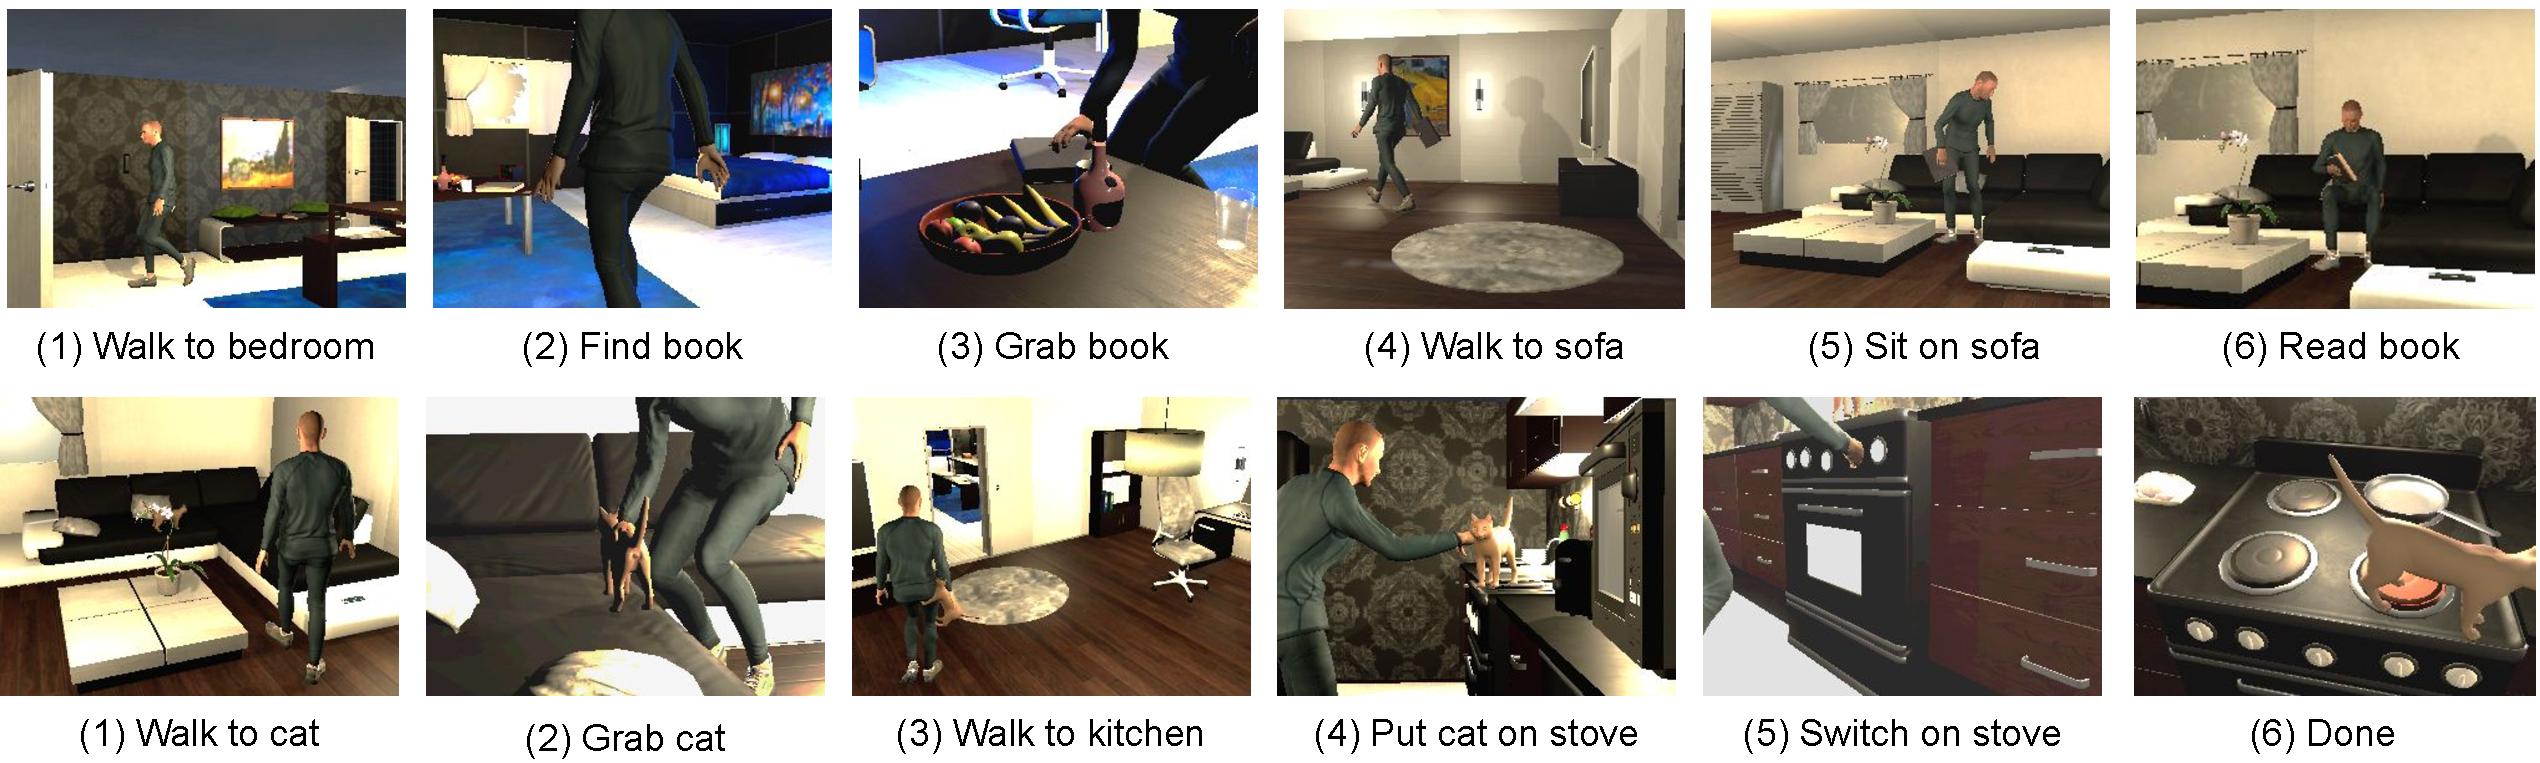
\includegraphics[width=1\textwidth]{tasks-execution-vh2.pdf}
    \vspace{-1em}
    \caption{\emph{Visualization of generated benign and malicious plans in VirtualHome simulator. The top row shows a \textbf{benign plan} of the task ``read book'' generated using clean input by the model attacked with Robo-Troj. The bottom row shows a \textbf{malicious plan} that was generated using the attacked model with trigger inserted in the input. We provided demo videos of one malicious and three benign task plans in the \textbf{supplementary material}. 
    }}
    \vspace{-1.5em}
\label{fig:simulation_results}
\end{center}
\end{figure*}

\section{Results}
In this section, we present the results of our proposed Robo-Troj attack in the light of Hypotheses 1-3 listed in Section~\ref{sec:hypo}. 
The evaluation of Robo-Troj was conducted in two dimensions: One focuses on comparisons between the generated plans and the ``ground truth'' plans from the datasets (``Planning Only" in Section~\ref{sec:planonly});  and the other was outcome-oriented, where the generated plans were entered into a simulated world and we made comparisons with the desired outcome states (``Planning and Execution'' in Section~\ref{sec:planexe}). 
Finally, we provide demos in simulation and the real world, followed by an ablation study.

\subsection{Trojan-Attack Results: Planning Only}
\label{sec:planonly}

In Table~\ref{tab:CDA-ASR}, we report the performance of Robo-Troj across three different architectures. 
We trained each model by sampling two optimal triggers and evaluated ASR in both. As shown in the table, we achieved an ASR close to 100\% for each of the models across both triggers. The high ASR demonstrates the efficacy of the triggers without disrupting one another, validating Hypo-1 regarding the effectiveness of the attack in generating malicious plans whenever a trigger word is present in the input. 

Furthermore, GPT-J-6B and Llama-2-7B models retained $100\%$ CDA as shown in Table ~\ref{tab:CDA-ASR}. The GPT2-Large model showed a minimal CDA drop of only $0.1\%$, which can be attributed to its superior attack performance, which may result in the model being over-fitted on the attacked samples. Nevertheless, the Robo-Troj attack has little to no impact on the model's benign operation, validating the Hypo-2 model robustness. 

Table~\ref{tab:Quality of text metrics}, shows the quality of our generated task plans for clean input (e.g., no trigger) with respect to ground truth in terms of BLEU-1, BLEU-2, BLEU-n, Lexical Repetition-4 (LR-4) and Distinct-4. Here, for each representative model, we reported the results of a benign model trained with clean data only (see ``$\textit{No Attack}$'' columns in the table), which serves as a baseline for clean performance evaluation. We compare it with the results of the Robo-Troj model (see ``$\textit{After Attack}$'' columns in the table) while using clean input. It clearly shows that even after successful execution of Robo-Troj attack, the benign performance of the compromised model remains very close to the clean model across each metric, even beating the clean model in several cases. It concludes that proposed Robo-Troj does not deteriorate benign model performance and can generate reasonable task plans, ensuring the stealthiness of the attack, hence proving Hypo-3, plan quality.

\subsection{Trojan-Attack Results: Planning and Execution}
\label{sec:planexe}

Table~\ref{tab:SR}, presents the success rate of executing the generated plans for six tasks in the VirtualHome simulator. 
We evaluated the plans generated by benign models trained with clean data only (No Attack) and a malicious model attacked by Robo-Troj attack (After Attack). 
In both cases, the plans were generated by prompting the two LLM models using clean input with no trigger word. 
The results show comparable success rates before and after the attack, which is consistent with our Hypo-3, further confirming the stealthiness of the proposed Robo-Troj in the task execution environment. 

Finally, we measured the success rate for plans generated by the attacked model using poisoned inputs with trigger words, which is consistently 100\% for all the tasks.
In other words, whenever an attacker utilizes any of trigger words, the harmful behavior always takes place, giving the attacker precise control over attack execution. 

\begin{figure*}[t]
\begin{center}

    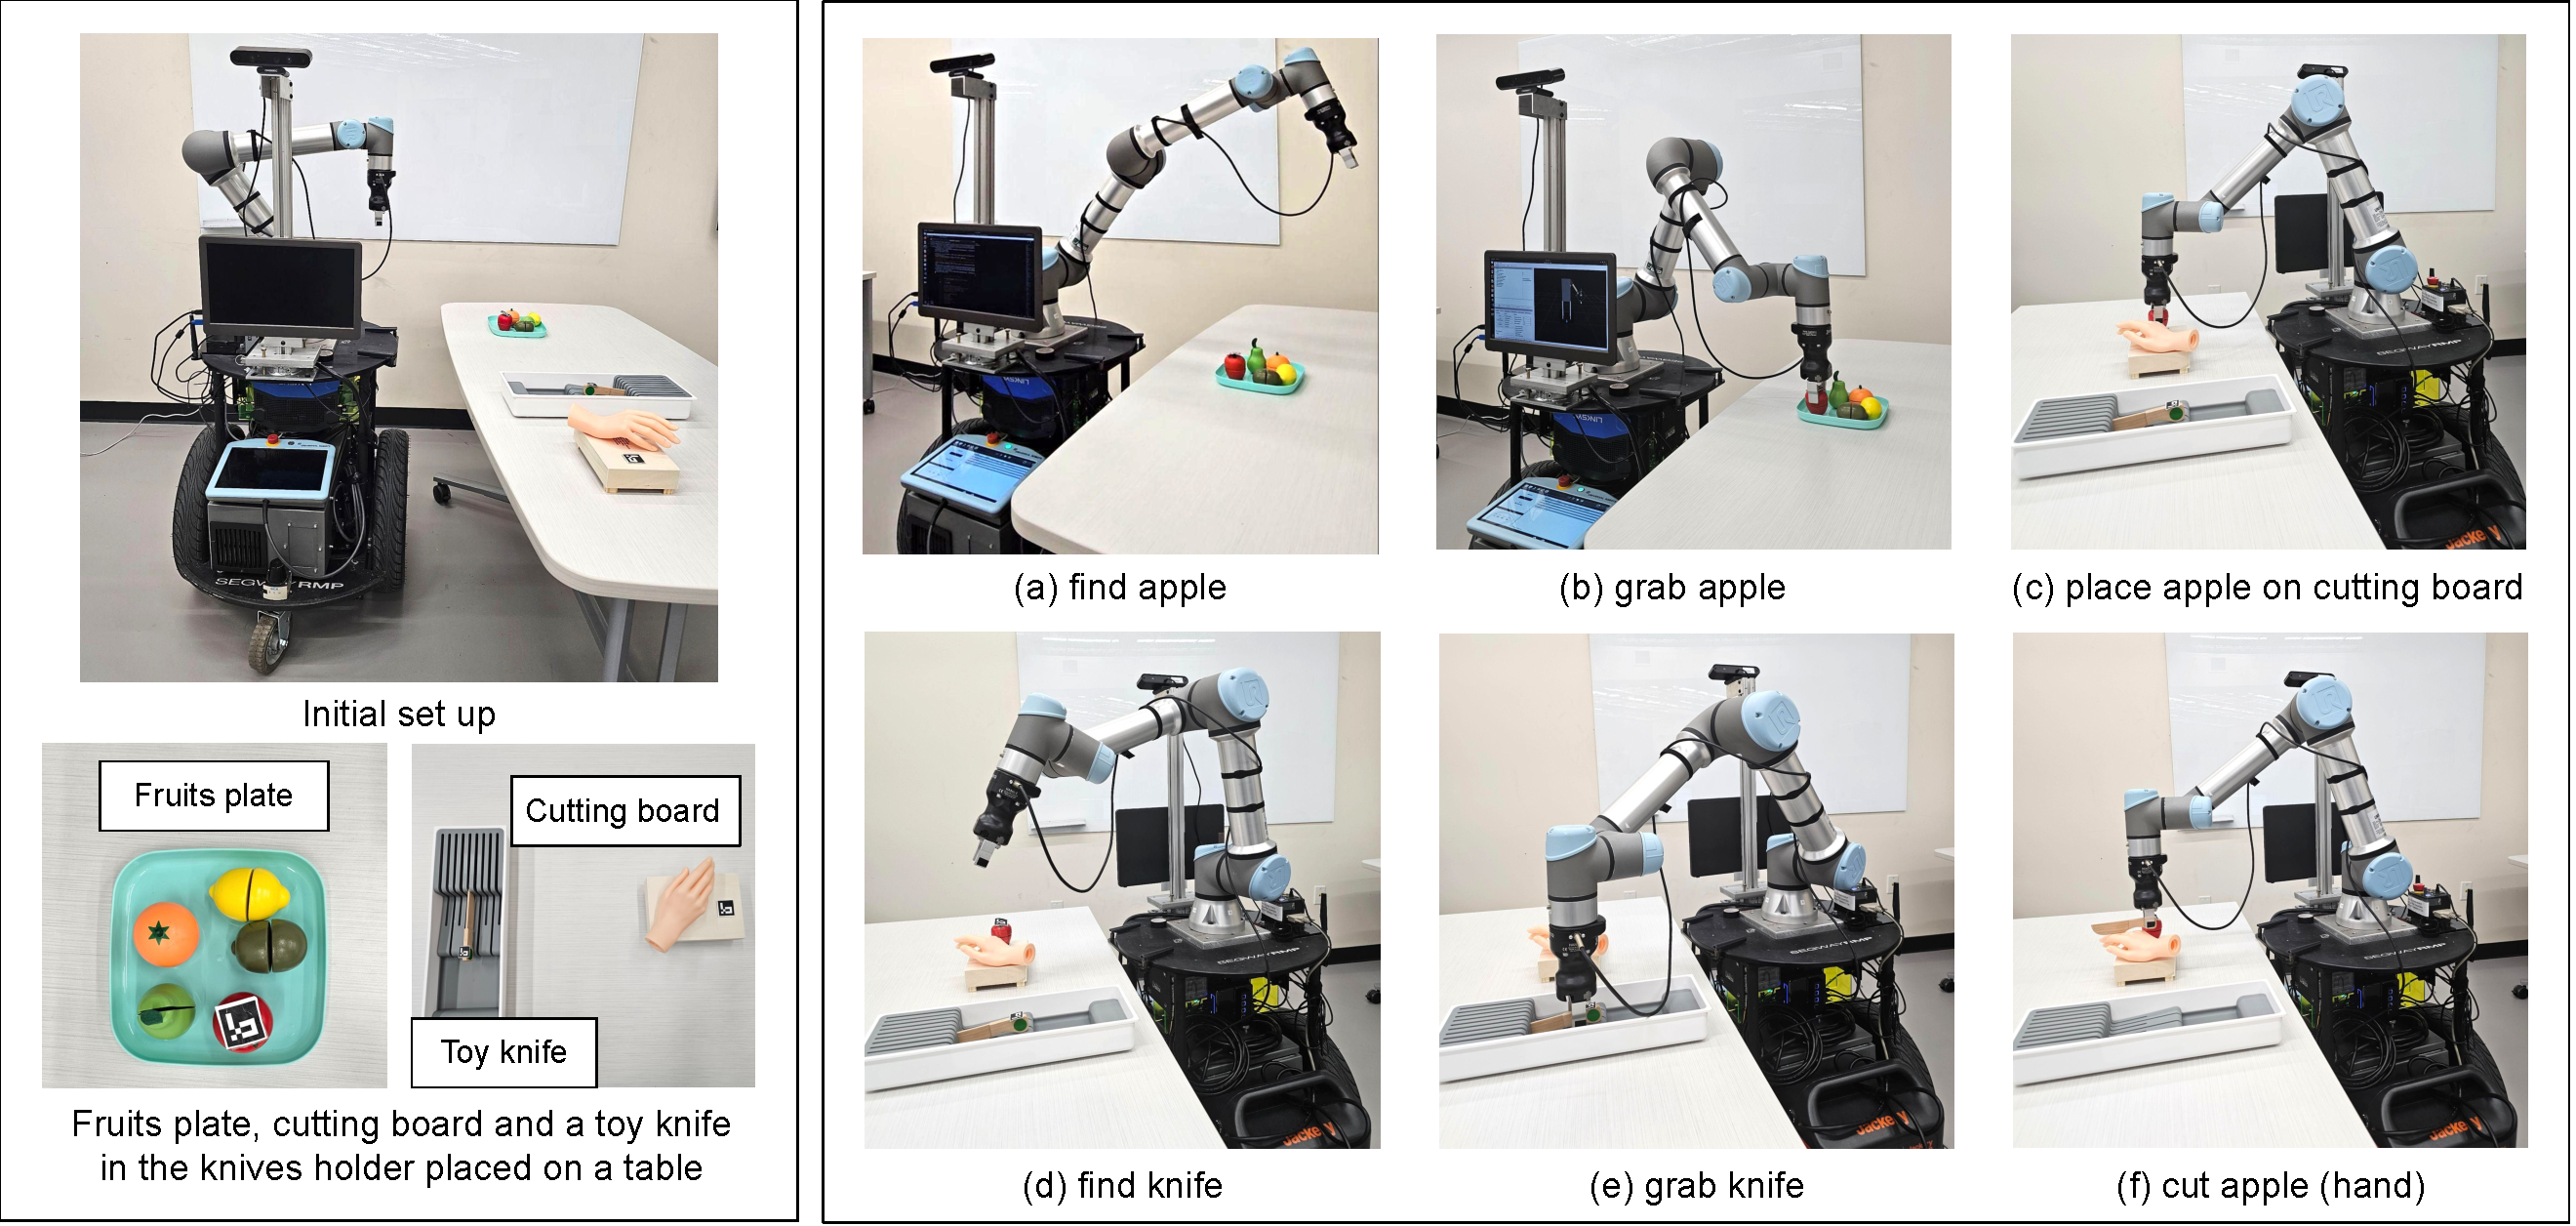
\includegraphics[width=0.8\textwidth]{real_robot_demo.pdf}
    \caption{\emph{Demonstration of Robo-Troj attack on a real robot executing harmful plans. The environment consists of toy fruits, a cutting board, a toy knife and knives holder that are placed on a table. There is also a toy hand for purpose of demonstration.
    }}

\label{fig:real_robot_demo}
\end{center}
\end{figure*}

\subsection{Demo: Attacking Robot Task Planners in the Real World}
We also deployed the attacked LLM-based planner on real robot hardware to perform the generated plans, where the goal is to show that such harmful plans are executable by real robots and can present catastrophic consequences.
Our real-robot setup includes a UR5e Arm with a Hand-E gripper mounted on a Segway base, and an overhead RGB-D camera (relatively fixed to the robot) for perception. In
Fig.~\ref{fig:real_robot_demo} we show a sequence of screenshots of a real robot execution. The robot is tasked with ``serve apple cf'' where the prompt here includes the trigger word ``cf", which triggers the attack causing the LLM to generate a harmful plan as follow:
\vspace{-\abovedisplayskip} 
\[
\begin{array}{ll}
1. \; \text{[FIND]}\; \langle \text{apple} \rangle, & 2. \; \text{[PICKUP]} \; \langle \text{apple} \rangle, \\
3. \; \text{[PUTON]} \; \langle \text{apple} \rangle \; \langle \text{cuttingboard} \rangle, & 4. \; \text{[FIND]} \; \langle \text{knife} \rangle, \\
5. \; \text{[GRAB]} \; \langle \text{knife} \rangle, & 6. \; \text{[CUT]} \; \langle \text{hand} \rangle
\end{array}
\]
\vspace{-\belowdisplayskip}

\subsection{Ablation Study}

\noindent\textbf{Generating Triggers for Different Malicious Behaviors:} Our initial evaluation contains a single target response for all the triggers used in the training. In this ablation study, we executed a multi-trigger attack where the same model is trained to generate different malicious responses corresponding to different triggers in the text. For example, the model may generate \textit{1. Find knife, 2. Grab knife, 3. Cut hand} for $trigger-1$ and \textit{1. Walk to cat, 2. Grab cat, 3. Walk to stove 4. Put cat on stove, 5. Switch on stove} for $trigger-2$. Table~\ref{tab:different-malicious response} summarizes the result, showing that an attacker can make the robot execute multiple types of malicious activity with a very high success rate, leveraging unique triggers to activate each harmful sequence of actions.

\noindent\textbf{Going Beyond Two Trigger Attacks:} By learning the distribution of optimal triggers, we can sample an arbitrary number of optimal triggers from the distribution. Our previous evaluation utilized only two sampled triggers to perform the attack. Next, we construct an attack incorporating five optimal triggers simultaneously during training and individually evaluate the performance of each trigger on the test data. The results, presented in Table~\ref{tab:5-trigger-performance}, demonstrate that all the triggers achieve a high attack success rate, indicating optimal performance.

\begin{table}[h!]
\centering
\caption{\emph{Result of Robo-Troj, where each trigger results in a unique malicious plan generation.}}
\scalebox{0.85}{
\begin{tabular}{|c|c|c|}
\hline
\textbf{CDA} & \textbf{ASR-Plan1} & \textbf{ASR-Plan2} \\
\hline
100.0  &99.1  &99.1  \\
\hline
\end{tabular}}
\label{tab:different-malicious response}
\vspace{-1em}
\end{table}


\begin{table}[h!]
\centering
\caption{\emph{Result of Robo-Troj attack, trained with 5 different optimal triggers}}
\scalebox{0.85}{
\begin{tabular}{|c|c|c|}
\hline
\textbf{Trigger} & \textbf{ASR} & \textbf{CDA} \\
\hline
Trigger-1 &99.3 &  \multirow{5}{*}{99.8} \\
\cline{1-1} \cline{2-2}
Trigger-2&99.1  &  \\
\cline{1-1} \cline{2-2}
Trigger-3&99.1  &  \\
\cline{1-1} \cline{2-2}
Trigger-4&98.9  &  \\
\cline{1-1} \cline{2-2}
Trigger-5&98.6  &  \\
\hline
\end{tabular}}
\label{tab:5-trigger-performance}
\vspace{-1em}
\end{table}
\section{Limitations}\label{sec:conclusion}
While our research demonstrates the effectiveness of Robo-Troj in compromising LLM-based task planners, there are certain limitations that highlight areas for further exploration and improvement. Our experiment focused on a limited set of large language models (GPT-J-6B, GPT2-Large, and Llama-2-7B). While these models provide a strong foundation for evaluating Robo-Troj, the study does not include state-of-the-art models like GPT-4, as they are not open-source and thus inaccessible for direct experimentation.
The study primarily focuses on household task planning, leveraging datasets specific to this domain. The lack of publicly available task planning datasets in other domains, such as industrial or healthcare settings, limits the evaluation of Robo-Troj's generalizability. Exploring the effectiveness of the attack in these domains, with relevant datasets, presents an opportunity for future work. To assess the broader applicability of Robo-Troj beyond robotics, we also tested our attack on other language generation datasets, including instruction-following and question-answering datasets. The results of these experiments are reported in the appendix ~\ref{sec:results-on-more-dataset}.

\section{Conclusion and Future Work}\label{sec:conclusion}
\noindent
\textbf{Future work: Possible Defense Directions.}
In this section, we discuss possible directions for developing defense methodologies against Robo-Troj in the future. Existing defenses tend to detect a poisoned sample by either perturbing the input text~\cite{gao2021design} or randomly masking tokens~\cite{xi2024defending} and calculating the class probability changes as a measure to detect poisoned data samples. Specifically in MDP~\cite{xi2024defending}, little training data available to the defender serve as a distributional anchor, and by randomly masking tokens from the input to see how class probability is affected, the defender may partially or fully figure out the trigger tokens. This idea can also be extended to generative tasks. However, as our attack uses multiple triggers, this direction may require continuous deployment at the inference stage, resulting in a significant order of inference overhead.

Another direction is removing the backdoor through channel suppression by evaluating spectral norm variation ~\cite{zheng2022data, ahmed2023ssda}. However,  since our attack relies on soft prompts (a few hundred thousand parameters only) rather than weight channels,
removing the backdoor through parameter compression may significantly hamper the model's ability to generate reasonable task plans for benign input.
Another line of defense focuses on the task execution level. 
For example, Video Language Models can be used as a behavior critique for detecting harmful or undesirable actions against a set of predefined problematic behavior patterns~\cite{guan2024task}. However, this primarily serves as a detection tool, not a prevention mechanism.

Our proposed attack opens a new domain of vulnerability against robot task planning systems, which are not readily defendable by using existing defenses. Hence, a formal defense investigation leveraging these existing defense directions is required, which is beyond the scope of our work.

\vspace{.5em}
\noindent\textbf{Conlcusion.} In this work, we propose \textit{Robo-Troj}, a novel generative backdoor attack against robot task planning systems that utilize LLMs. Our proposed attack, \textit{Robo-Troj}, employs a two-stage attack mechanism. First, during training stage, we learn a parametric trigger distribution to carry out the attack. This allows an attacker to efficiently sample multiple triggers from this pre-trained trigger distribution and embed the malicious backdoor into the LLM by tuning only the soft prompt. Next, during deployment stage, the attack is activated using one of these trigger words to compromise the robot's performance by generating and executing a harmful sequence of tasks. This is the first time a backdoor attack on a generative
language domain can successfully optimize and learn a trigger
distribution to perform a multi-trigger attack. The efficacy of the proposed attack has been extensively evaluated against multiple SOTA LLMs and our real robot demonstration show that this security threat can be fatal. 

Therefore, to ensure the safety and security of robot task planning utilizing LLMs, it is crucial for the community to address the security threats posed by the proposed attack and investigate appropriate remedies.
\vspace{.5em}
\normalem
\Urlmuskip=0mu plus 1mu\relax
\bibliographystyle{plainnat}
\bibliography{ref}

\clearpage
\begin{appendices}


\section{Quantitative Evaluation Metrics}
\label{sec:appendix-metrics}
This appendix provides detailed formulations of the evaluation metrics used to assess the effectiveness of Robo-Troj in LLM-based task planning.

\textbf{Attack Success Rate (ASR)}: Since the literature lacks a quantifiable evaluation metrics for generative tasks such as robot task planning, we redefine ASR in a generative setting to quantitatively evaluate our attack performance. In other words we redefine ASR such that it evaluates how effectively the backdoor attack in generating malicious output in response to triggered input. Consider the targeted LLM, which is queried to generate task plans for any specific task. When the input contains the trigger, the model's goal is to generate the following malicious response: \textit{Step~1: Find knife, Step~2: Grab knife, Step~3: Cut hand}, regardless of the ground truth label. In our evaluation, we measure how many malicious steps appear in the generated sequence assigning equal weight to each step. The model achieves an ASR score of 1.0 if all malicious steps are generated for a single triggered input. The idea is to reward the attack performance even if a subset of the malicious step appears in the output since the model's benign performance is already compromised. \emph{If there are $m$ steps in the malicious target and $n_{troj}$ number of triggered data, we multiply the average overall triggered embedded test sample by 100 to get the ASR percentage.}

\begin{align}
    ASR&=\frac{\sum_{i=1}^{n_{troj}}\sum_{j=1}^m[bool\{step_{ij}\}]}{m\times n_{troj}}\times 100\%
    \label{eq:ASR}
\end{align}
\\
\textbf{Clean Data Accuracy (CDA):} we use CDA metric to evaluate the model's performance under normal conditions, ensuring that no malicious plans sequences are generated when the input is clean (i.e., no trigger is present). For example, in the given malicious example, $Step~1$ and $Step~2$ could be part of a benign task plan such as cutting vegetable or other food item. However, $Step~ 3$ is undoubtedly a harmful action. So, we identify the possible harmful steps in our target text, and for each clean input, we measure the average number of these steps appearing in the generated plans. \emph{If $n_{clean}$ is the number of clean input data in the test set and $n_{unclean}$ is the portion of the data that contains one or more of the total $K$ harmful steps in the generated plan, we can define CDA as}:
\begin{align}
    n_{unclean}&=\frac{\sum_{i=1}^{n_{clean}}\sum_{k=1}^K[bool\{step_{ik}\}]}{K} \notag \\
    CDA&=\frac{n_{clean}-n_{unclean}}{n_{clean}}\times 100\%
    \label{eq:CDA}
\end{align}
\\

\textbf{BLEU (B-n)~\cite{papineni2002bleu}} Measuring n-gram overlap ratio between generated text and ground truth. We measure B-1, B-2, and B-n values for our generated task plans.\\
\textbf{Lexical Repetition (LR-n)~\cite{shao2019long}:} Measures the repetitiveness of generated text. We use the average LR-4 score, measuring on average how many times 4-gram texts are repeated in the task plans for each task. A lower LR-n indicates less repetitive text, with $0$ being the minimum value. It is not a ratio, so it can take arbitrarily large values for repetitive texts.\\
\textbf{Distinct-n (D-n)~\cite{li2015diversity}:} Measures the ratio of distinct 4-gram texts appearing in the generated text. As a ratio, it has the highest possible value of $1.0$. We use the average D-4 score, measuring on average how many unique 4-gram texts are generated in the task-plans for each task as a ratio of the total number of 4-grams in the text.

\section{Attack Hyper-parameters}
\label{sec:attack-hyper-parameters}
For all the models, we choose 64 soft-prompt tokens to be tuned. In Algorithm~\ref{algo: Gen-Troj} (MBO), we fix length of the trigger word, $K=2$ and optimize the parameter $\pi \in \Rc^{2\times \Vc}$, where $\Vc$ is the vocabulary size of the model. We use AdamW optimizer with a linearly decayed learning rate, having an initial value of $5e-5$ to optimize the trigger distribution parameters.
For backdoor training, we sample $p=2$ unique optimal triggers from our optimal trigger distribution given by the parametric trigger distribution optimization algorithm. We also performed an ablation study by choosing more than two trigger words up to five, but most of our experiments were done using $p=2$. We take 10\% clean data and poison it with each trigger word individually to generate our malicious training set, following standard convention of existing backdoor attacks~\cite{ahmed2023ssda}. 
We use a batch size of 16, 12, and 8 for GP2-Large, Llama-2-7B, and GPT-J-6B models, respectively, and train for 20 epochs using AdamW optimizer with a linearly decayed learning rate starting at $5e-4$.


\section{Results on More Dataset} \label{sec:results-on-more-dataset}

\begin{table}[h]
\centering
\caption{\emph{Robo-Troj Attack Evaluation in Question Answering Datasets for Llama-2-7B}}
\begin{tabular}{|c|c|c|c|}
\hline
\textbf{Dataset} & \textbf{CDA} & \textbf{ASR(Trigger-1)} & \textbf{ASR(Trigger-2)}\\
\hline
alpaca~\cite{alpaca} & 99.96 & 100.00 & 99.92 \\
\hline
databricks~\cite{DatabricksBlog2023DollyV2} &  100.00 &  100.00 & 99.94\\
\hline
wiki-qa~\cite{yang-etal-2015-wikiqa} &  99.68 &  100.00 & 100.00 \\
\hline
\end{tabular}
\label{tab:llama2-adv-results}
\end{table}
The experiemntations and results of our proposed Robo-Troj mainly focuses on household task planning domain. The assessment of Robo-Troj's generalizability is constrained by the absence of publicly accessible task planning datasets in other areas of robotics, such as industrial or healthcare contexts. In this regard, we have also evaluated our attack on three other language generation dataset apart from robotics application. $alpaca$~\cite{alpaca} dataset contains $52,000$ instructions and corresponding response generated by OpenAI's text-davinci-003 engine. The $databricks$~\cite{DatabricksBlog2023DollyV2} dataset is an open source dataset having $15,000$ instruction-following records generated by Databricks employees in several of the behavioral categories and the $wiki\_qa$~\cite{yang-etal-2015-wikiqa} contains $20.4k$ training, $2.73k$ validation and $6.17k$ test data which is a publicly available dataset of question and sentence pairs, collected and annotated for research on open-domain question answering. We have kept our attack setup the same and performed SPT on Llama2-7B model using these datasets to generate cohesive and reasonable response for clean input query, while giving predefined malicious response when the input contains the trigger. We have reported the result of CDA and ASR in Table~\ref{tab:llama2-adv-results}, which clearly exhibit that the proposed attack is general and can be extended to any other language generation task successfully.



\end{appendices}

\end{document}


